\section{Demand Characterization of an Engine Control Tasks}   \label{chap:codesign}

\subsection{Introduction}

Resource management is a key consideration in any real-time system.
Pessimistic assumptions lead to overestimation of workload, which results in underutilization of the resources. On the other hand, workload underestimation can cause deadline misses.
For a system with hard real-time requirements, missing deadlines can be catastrophic.
An example is the powertrain control module (PCM) of a car \cite{noauthor_electricalelectronic_2008}. 
The ignition system and fuel injection tasks, which are managed by the PCM, are initiated based on the crankshaft's relative position with respect to fixed points in its path of rotation. 
%A task can have one or multiple job releases in a single rotation. 
As the crankshaft's angular speed increases, the crankshaft reaches a given angle faster, hence increasing the number of job releases in a given time interval.
As a result, at higher speeds, a larger number of jobs are released, and if not properly scheduled, some jobs could miss their deadlines.

An engine's behavior is generally more stable at higher speeds due to frequent sensor and actuation updates. Hence, jobs released at higher speeds may have lower execution times~\cite{dbuttle_real-time_nodate}.
To reflect this, the so-called engine-triggered tasks are modeled to have smaller execution times as the speed increases.
In addition, as the speed increases, the time taken to complete a rotation decreases and hence the inter-arrival time between two consecutive jobs also decreases.
Since the traditional periodic task model~\cite{liu_scheduling_1973} assumes a constant time period for a task, applying it to define systems such as a vehicle with PCM would result in overly pessimistic utilization.
To tackle this, a model called the adaptive variable rate (AVR) task model has been proposed to capture the behavior of engine-triggered tasks.
An AVR task is defined by a set of modes, each of which is expressed by a range of speeds~\cite{dbuttle_real-time_nodate} and a constant execution time as shown in Fig.~\ref{fig:AVRImage}.

To determine whether an AVR task is schedulable using EDF, the demand bound function (\dbf) is often used~\cite{biondi_response-time_2015,biondi_feasibility_2015} to measure the resource requirement over a given time interval. In a nutshell, \dbf~ determines the worst-case aggregate execution time of the jobs that have both the arrivals and deadlines within a time interval $[t_1,t_2]$.
In general, the calculation of the worst-case demand of an AVR task is not straightforward.
%Let us consider the example in Fig.~\ref{fig:AVRImage}. 
Let us consider an example.
In a time interval $[t_1,t_2]$, assume 15 jobs are released at the highest allowable speed with each job having an execution time of \unit[50]{$\mu s$}.
On the other hand, during the same duration, assume 10 job releases are possible at the lowest speed with each job having an execution time of \unit[100]{$\mu$s}.
The demand when the jobs are released at the lowest speed (\unit[1,000]{$\mu$s}) is greater than when the jobs are released at the highest speed (\unit[750]{$\mu s$}).
Suppose instead that the jobs that are released at the highest speed have an execution time of \unit[70]{$\mu s$}.
In this case, the demand of these jobs is greater than the demand of the jobs that are released at the lowest speed. 
%10 jobs are released at the highest speed and 4 job releases are possible at the lowest speed, during the same time interval, the demand is higher in the former case. 
Hence, the demand depends on the relationship between the task's execution times and speeds, as well as the acceleration profiles of the engine.  

\begin{figure}
\centering
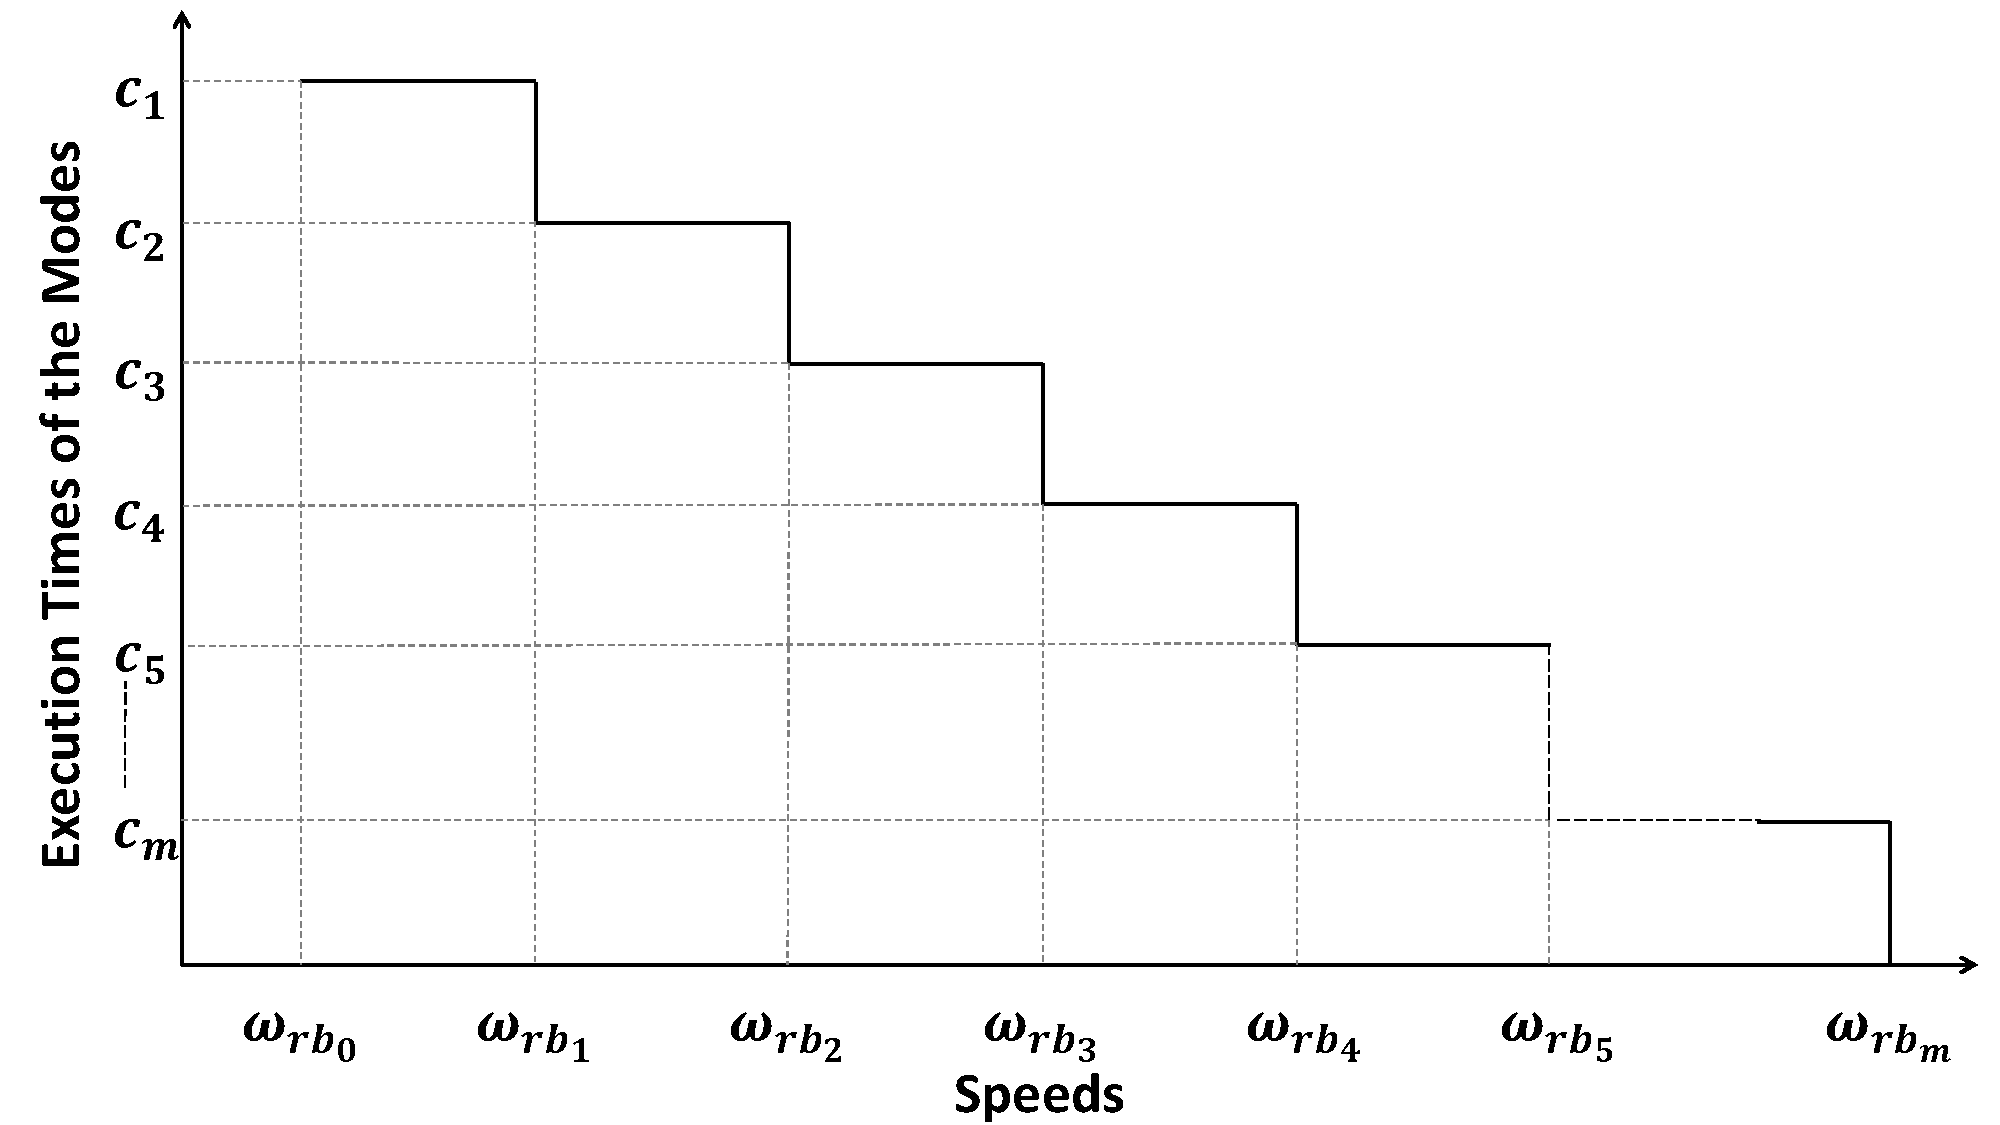
\includegraphics[width=\linewidth]{Figures/AVRImage.pdf}
\caption{Different modes of an AVR task where $c_i$ and $\omega_{rb_i}$ are the execution time and the right boundary speed of the $i^{\rm th}$ mode, respectively.}
\label{fig:AVRImage}
\end{figure}

Several methods have been proposed to calculate the \dbf~of an AVR task.
Mohaqeqi et al.~\cite{mohaqeqi_refinement_2017} proposed an exact analysis, using the Digraph model~\cite{stigge_digraph_2011}, to transform an AVR task into a digraph to calculate the exact worst-case demand assuming that the crankshaft can have multiple acceleration values during a rotation.
While this approach represents the state-of-the-art technique, it is computationally intensive and unlikely to be suitable for large problem instances.
In this paper, we propose a knapsack-based method to efficiently calculate the exact worst-case demand of an AVR task.

\noindent \textbf{Contributions}: The main contributions of this paper are:
\begin{enumerate}
\item To determine the worst-case demand of an AVR task, the search for the dominant job sequence, i.e., one that results in the maximum demand over a given time interval, is modeled as a bounded precedence constraint knapsack problem.
A dynamic programming based approach is presented to exactly and efficiently solve the problem.
\item  The number of job sequences that need to be considered when calculating the worst-case demand of an AVR task is significantly reduced by exploiting the kinematic properties of the engine.
\item Experimental results based on existing AVR task sets as well as randomly generated AVR task sets reveal that the proposed approach significantly outperforms the state-of-the-art technique~\cite{mohaqeqi_refinement_2017} in terms of computation time.
\end{enumerate}

The rest of the paper is organized as follows.
In Section~\ref{sec:relatedWork}, we review key existing work pertaining to AVR tasks.
In Section~\ref{sec:prelims}, we introduce the system model, discuss our assumptions and formally present the problem.
In Section~\ref{sec:knapsack}, we present a knapsack-based approach to find the worst-case demand of AVR tasks. %...using the aforementioned dominant sequence set.
We provide some necessary conditions to reduce the search space in Section~\ref{sec:filterSeq} and describe the dominant sequence set in Section~\ref{sec:Summary}.
Experimental results are presented in Section~\ref{sec:experimental} and the paper concludes in Section~\ref{sec:conclusion}.

\subsection{Preliminaries}
\label{sec:prelims}

In this section, we provide some background materials on the engine and its properties and introduce our task model.
We also formally define the problem.
\paragraph{Task Model}
Adaptive variable rate (AVR) tasks are triggered at certain angles with respect to the top dead center position of the crankshaft, unlike periodic tasks which release jobs at regular time intervals.
For example, consider the different stages of fuel ignition in a vehicle as shown in Fig.~\ref{fig:Engine}.
For optimal performance of the engine, fuel injection should occur at a precise angle.
As the rate of arrival of the crankshaft at a given angle varies with its angular speed, AVR tasks do not have a fixed period.
Rather, at a higher speed, a larger number of instances (i.e., jobs) of each task occur, potentially increasing the resource requirement.

While it is possible to determine the schedulability of a task set assuming that this increased resource requirement of an AVR task is its steady-state demand, doing so would lead to pessimistic analyses and hence resource underutilization.
Moreover, the engine is more stable at higher speeds~\cite{dbuttle_real-time_nodate}.
This allows jobs to have shorter execution times at higher crankshaft speeds.
Hence, the execution time of AVR tasks is modeled as a function of the speed at which the jobs are released, as shown in Fig.~\ref{fig:AVRImage}.

%PNG Graphic
%\begin{figure}
%\centering
%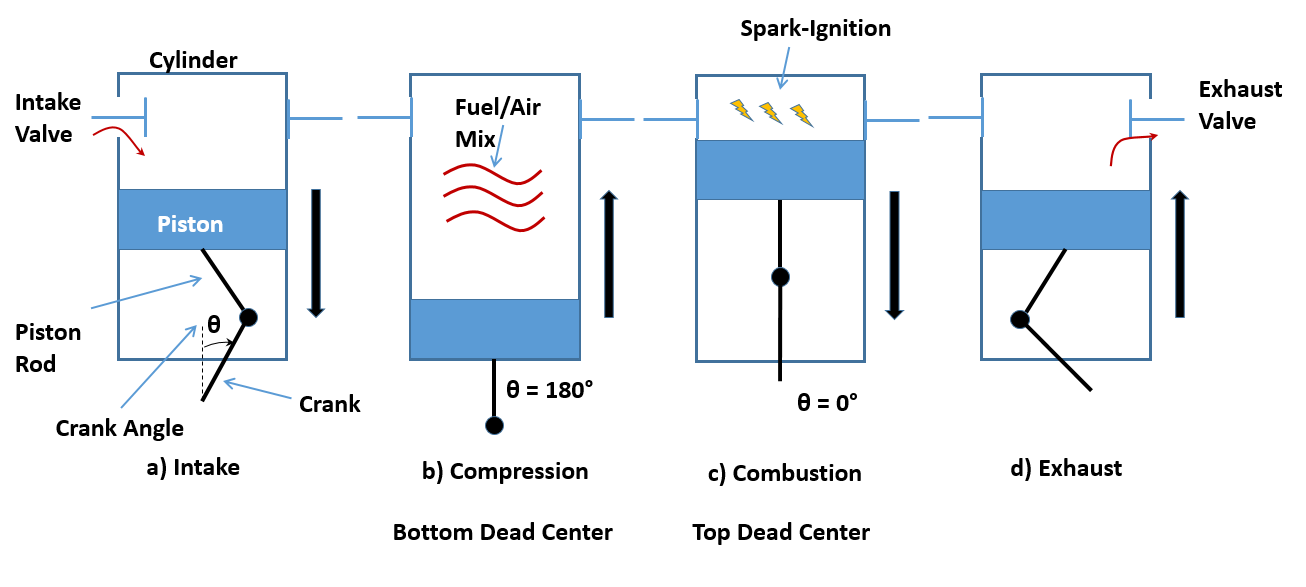
\includegraphics[width=\linewidth]{Figures/Engine.PNG}
%\caption{Different stages of fuel ignition in a vehicle.}
%\label{fig:Engine}
%\end{figure}

%Vector Graphic - Last Update: 2018-08-21-12:05 - Aaron
\begin{figure}
    \centering
    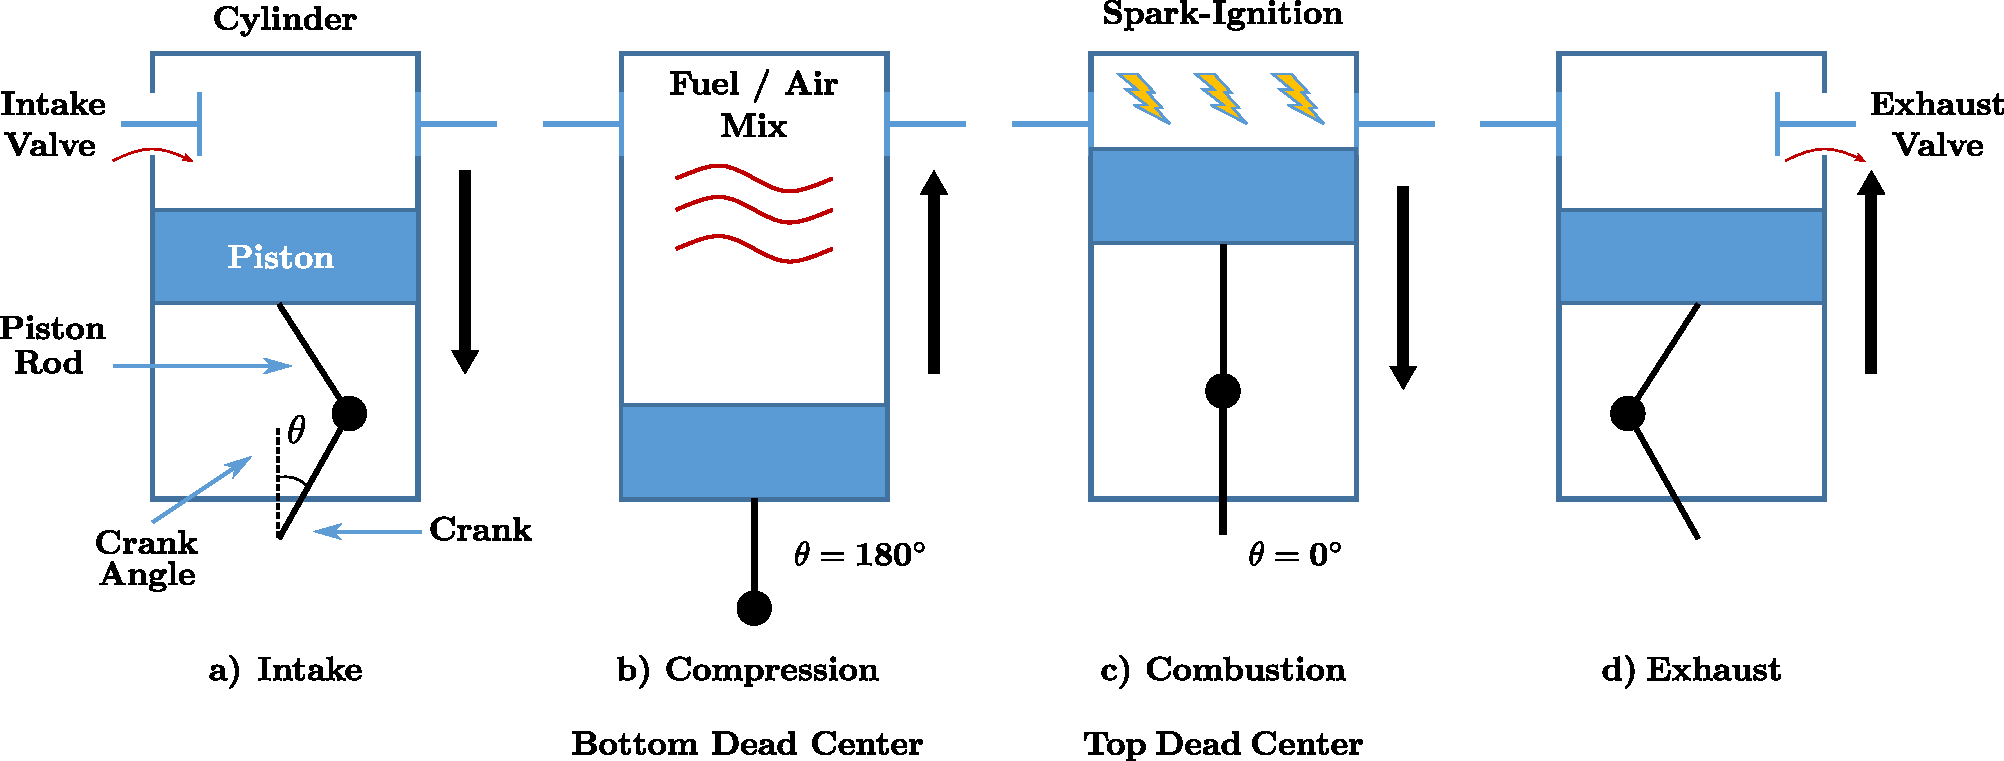
\includegraphics[width=0.9\linewidth]{Figures/vectorEngineIsolated.pdf}
    \caption{Different stages of fuel ignition in a vehicle.}
    \label{fig:Engine}
\end{figure}

%An AVR task is typically modeled as a decreasing staircase function as shown in Fig.~\ref{fig:AVRImage}. 
The range of speeds in which the execution time is constant is referred to as a mode and the edge speeds of the mode are referred to as the \emph{boundary speeds} of the mode.
The set of speeds where the mode changes are defined as the set of right boundary speeds, i.e., $\mathbf{\Omega_{rb}}=\{\omega_{rb_1}, \ldots, \omega_{rb_{m}} \}$, 
$\forall \omega \in (\omega_{rb_{i-1}},\omega_{rb_i}]$, speed $\omega$ is in the $i^{\rm th}$ mode. 
%The right boundary speed of the $i^{\rm th}$ mode is represented as \(\omega_{rb_i}\).   
We further define $\mathbf{\Omega_{rb}}(\omega)$ to be all the right boundary speeds larger than $\omega$ that are reachable (defined later in Section~\ref{sec:prelims}). 
%As the staircase function is made of a series of steps, we use the terms steps and modes interchangeably. 
%\sandeep{If we don't use steps , we can remove this.}
The minimum and maximum allowable speeds of rotation of the crankshaft are represented by \(\omega_{rb_0}\) and \(\omega_{rb_m}\) respectively.
 For convenience, we refer to %these special right boundary speeds 
them as $\omega_{\min}$ and $\omega_{\max}$, respectively and assume $\omega \geq 0, \, \forall \omega \in [\omega_{\min},\omega_{\max}]$, where $\omega$ is assumed to be in $\text{rev/min}$.
In addition, the instantaneous speed at a given time $t$ is denoted as $\omega(t)$. %Alternatively, we also use the notation $\omega_\ell$ to represent the crankshaft speed at time $t_\ell$.
A table of notations can be found in Appendix \ref{appendix:engCtrl-table-of-notation}.

The maximum allowable acceleration and deceleration are denoted by \(\alpha_{\max}\) and \(\alpha_{\min}\), respectively, both assumed to be in $\text{rev/min}^2$.
In this paper, we assume $\alpha_{max}=|\alpha_{min}|$.
The execution time of the $i^{\rm th}$ mode is represented by $c_i$.
Additionally, the execution time corresponding to a speed $\omega(t)$, is denoted by $c(\omega(t))$.
We assume that a job is released at the top dead center position, which we consider as the beginning of the rotation.
Thus, a job's execution time is determined by the speed of the crankshaft at the beginning of its the rotation.

\begin{property}[Speed After $n$ Rotations]
Given an initial speed of $\omega(t)$ at time $t$ and a constant acceleration $\alpha$,
the speed after an angular displacement of $\Delta \theta$
is~\cite{verma_concepts_nodate, biondi_exact_2014}
\begin{equation}
\label{eqn:rotation}
    \Omega(\omega(t),\alpha, \Delta \theta) = \sqrt[]{\omega(t)^2+2\alpha \Delta \theta}.
\end{equation}

Similar to the work by Mohaqeqi et al.~\cite{mohaqeqi_refinement_2017} we assume that $\Delta \theta$ specifies the crankshaft revolution in terms of the number of rotations, i.e., $ \Delta \theta = 1$ indicates a complete rotation.
Hence, according to Equation~\ref{eqn:rotation}, assuming an initial speed of $\omega(t)$ at time $t$, and a constant acceleration of $\alpha$, the speed after one complete rotation is $\Omega_1(\omega(t),\alpha) = \sqrt[]{\omega(t)^2+2\alpha}$.
In general, the speed after $n$ complete rotations is~\cite{mohaqeqi_refinement_2017},
\begin{equation}
\label{eqn:rotation-n}
    \Omega_n(\omega(t),\alpha) = \sqrt[]{\omega(t)^2+2 n \alpha}.
\end{equation}
\end{property}


Biondi et al. \cite{biondi_response-time_2015} showed that multiple AVR tasks activated by the same source and, which have the same angular phase and period can be modeled as a single AVR task, called the representative AVR task.
Hence, the analysis in this paper can also be extended to multiple AVR tasks.


\paragraph{Minimum Job Inter-arrival Times}

The minimum inter-arrival time is the minimum time duration from the release of a job at $t_1$ when the speed is $\omega(t_1)$ to the next job release at $t_2$ and speed $\omega(t_2)$. We denote minimum inter-arrival time by $\widetilde{T}(\omega(t_1),\omega(t_2))$.
In order to overcome the drawback of using constant acceleration between job releases as was assumed in most existing work~\cite{biondi_response-time_2015,biondi_feasibility_2015,biondi_exact_2014}, we consider the possibility of acceleration variations between two job releases similar to the work by Mohaqeqi et al.~\cite{mohaqeqi_refinement_2017}.

The minimum inter-arrival time equation by Mohaqeqi et al.~\cite{mohaqeqi_refinement_2017} is briefly presented here using simplified notation for readability.
To get the minimum inter-arrival time from any speed $\omega$, the crankshaft has to be maximally accelerated from $\omega$ to reach $\omega_{p}$, the peak speed, and then maximally decelerated to reach a target speed $f$ in a single rotation,
% \begin{equation}\label{eq:peakSpeed}
% \omega_{peak} = \sqrt{\frac{2\alpha_{\min}\alpha_{\max}+\alpha_{\min}\omega(t_1)^2-\alpha_{\max}\omega(t_2)^2}{\alpha_{\min} - \alpha_{\max}}}.
% \end{equation}
\begin{equation}\label{eq:peakSpeed}
\omega_p(\omega,f) = \frac{\sqrt{2\omega^2 + 2f^2 + 2\alpha_{\max}}}{2}.
\end{equation}

However, if $\omega_{p}>\omega_{max}$, the crankshaft has to maximally accelerate from $\omega$ to $\omega_{max}$, stay at that speed for some time and then maximally decelerate to $f$.
The two cases are defined below and presented in Figure \ref{fig:mint}:
% \begin{alignat}{3}\label{minTime}
%     &\widetilde{T}(\omega(t_2),\omega(t_1)) = \nonumber &\\
%     &\left\{
%         \def\arraystretch{2.0} %Switch to 2.2 for best results
%         \begin{array}{ll}
%             \frac{\omega_{rb_m}-\omega(t_1)}{\alpha_{max}} 
%             + \frac{\omega(t_2) - \omega_{rb_m}}{\alpha_{min}} +\frac{1}{\omega_{rb_m}} \cdot \\ \bigg(1-\frac{\omega_{rb_m}^2-\omega(t_1)^2}{2\alpha_{max}}           -\frac{\omega(t_2)^2-\omega_{rb_m}^2}{2\alpha_{min}} \bigg)
%             & \omega_{peak} > \omega_{\max} \\
%             \frac{\omega_{peak}-\omega(t_1)}{\alpha_{\max}} + \frac{\omega(t_2)-\omega_{peak}}{\alpha_{\min}} & \omega_{peak} \leq \omega_{\max}
%         \end{array}
%     \right.
% \end{alignat}
\begin{alignat}{3}\label{eq:minTime}
  &\widetilde{T}(\omega,f) = \\
  &\left\{
        \def\arraystretch{2.0}
        \begin{array}{ll}
            \frac{\sqrt{2\omega^2+2f^2+4\alpha_{\max}}-\omega-f}{\alpha_{\max}} & \ \omega_p(w,f) \leq \omega_{\max} \ \\
            \frac{\omega_{max} - f - \omega}{\alpha_{\max}} + \frac{\omega^2 + f^2}{2\omega_{\max}\alpha_{\max}}+\frac{1}{\omega_{\max}} & \ \omega_p(w,f) > \omega_{\max}
        \end{array}
    \right. \nonumber
\end{alignat}

\begin{figure}
\centering
  \subfloat[$\widetilde{T}(\omega,f) | \omega_{p}(\omega,f) \leq \omega_{\max}$]{
      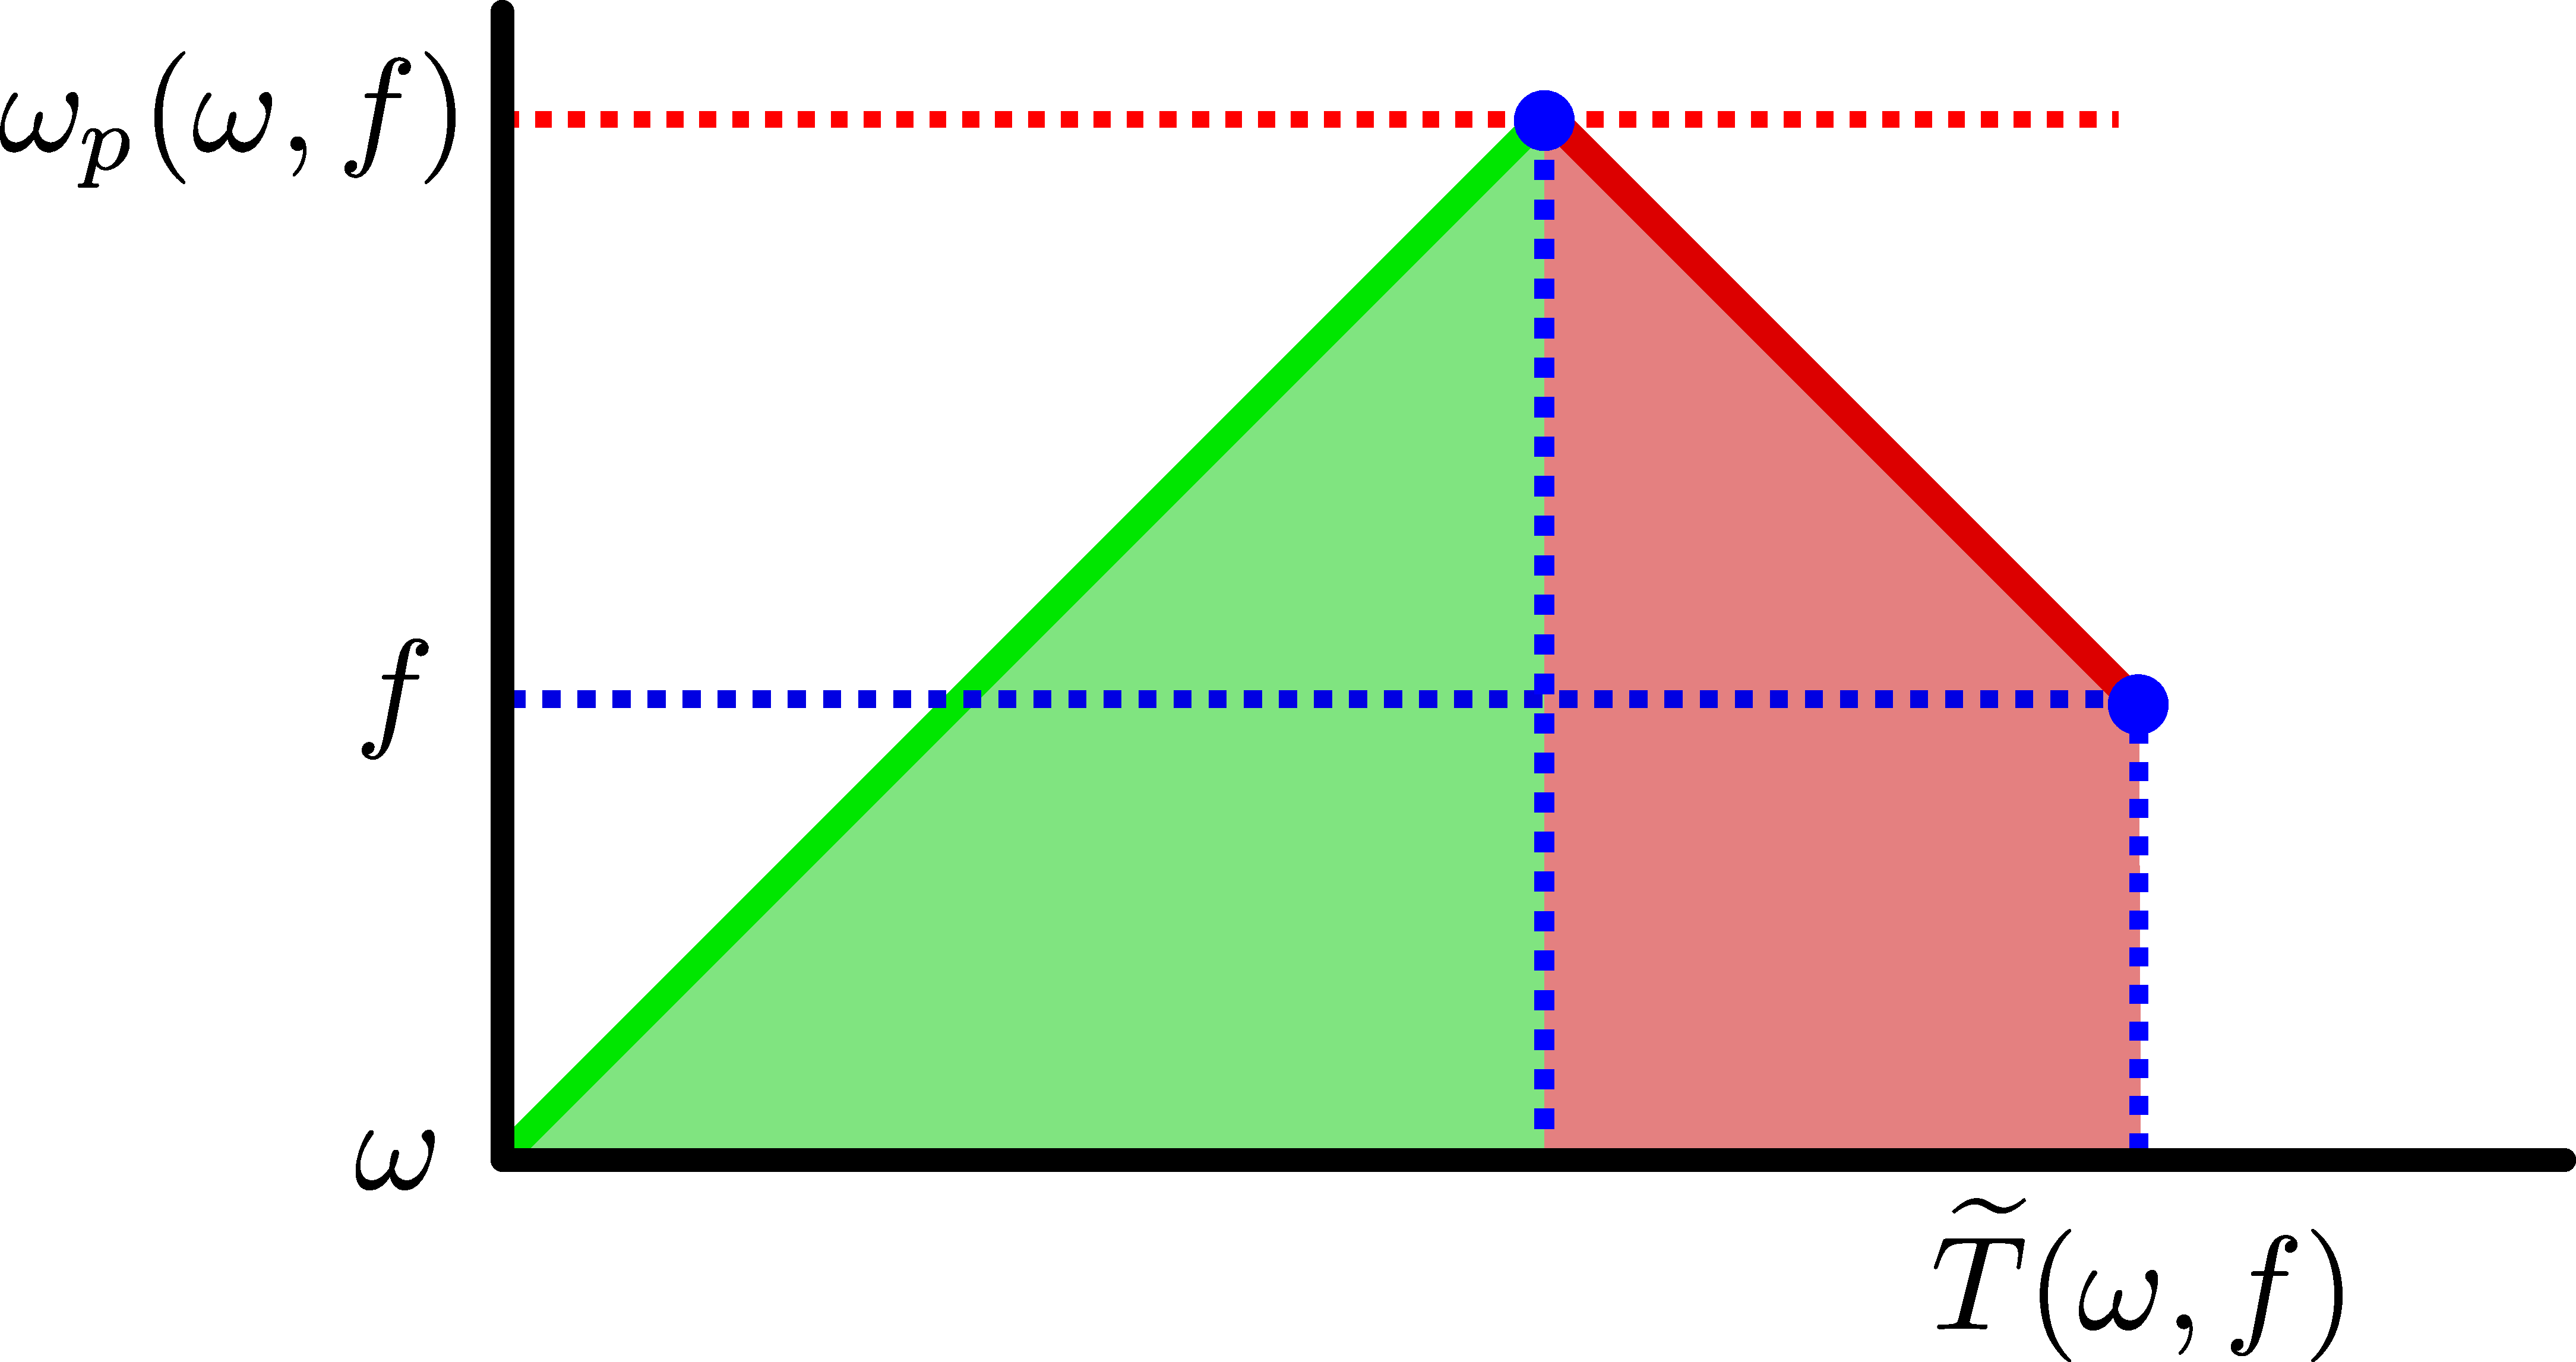
\includegraphics[scale=0.055]{Figures/mint-peakBare.pdf}}
      \label{fig:mintPeak}
  \label{mintPeak}
  \subfloat[$\widetilde{T}(\omega,f) | \omega_{p}(\omega,f) > \omega_{\max}$]{
      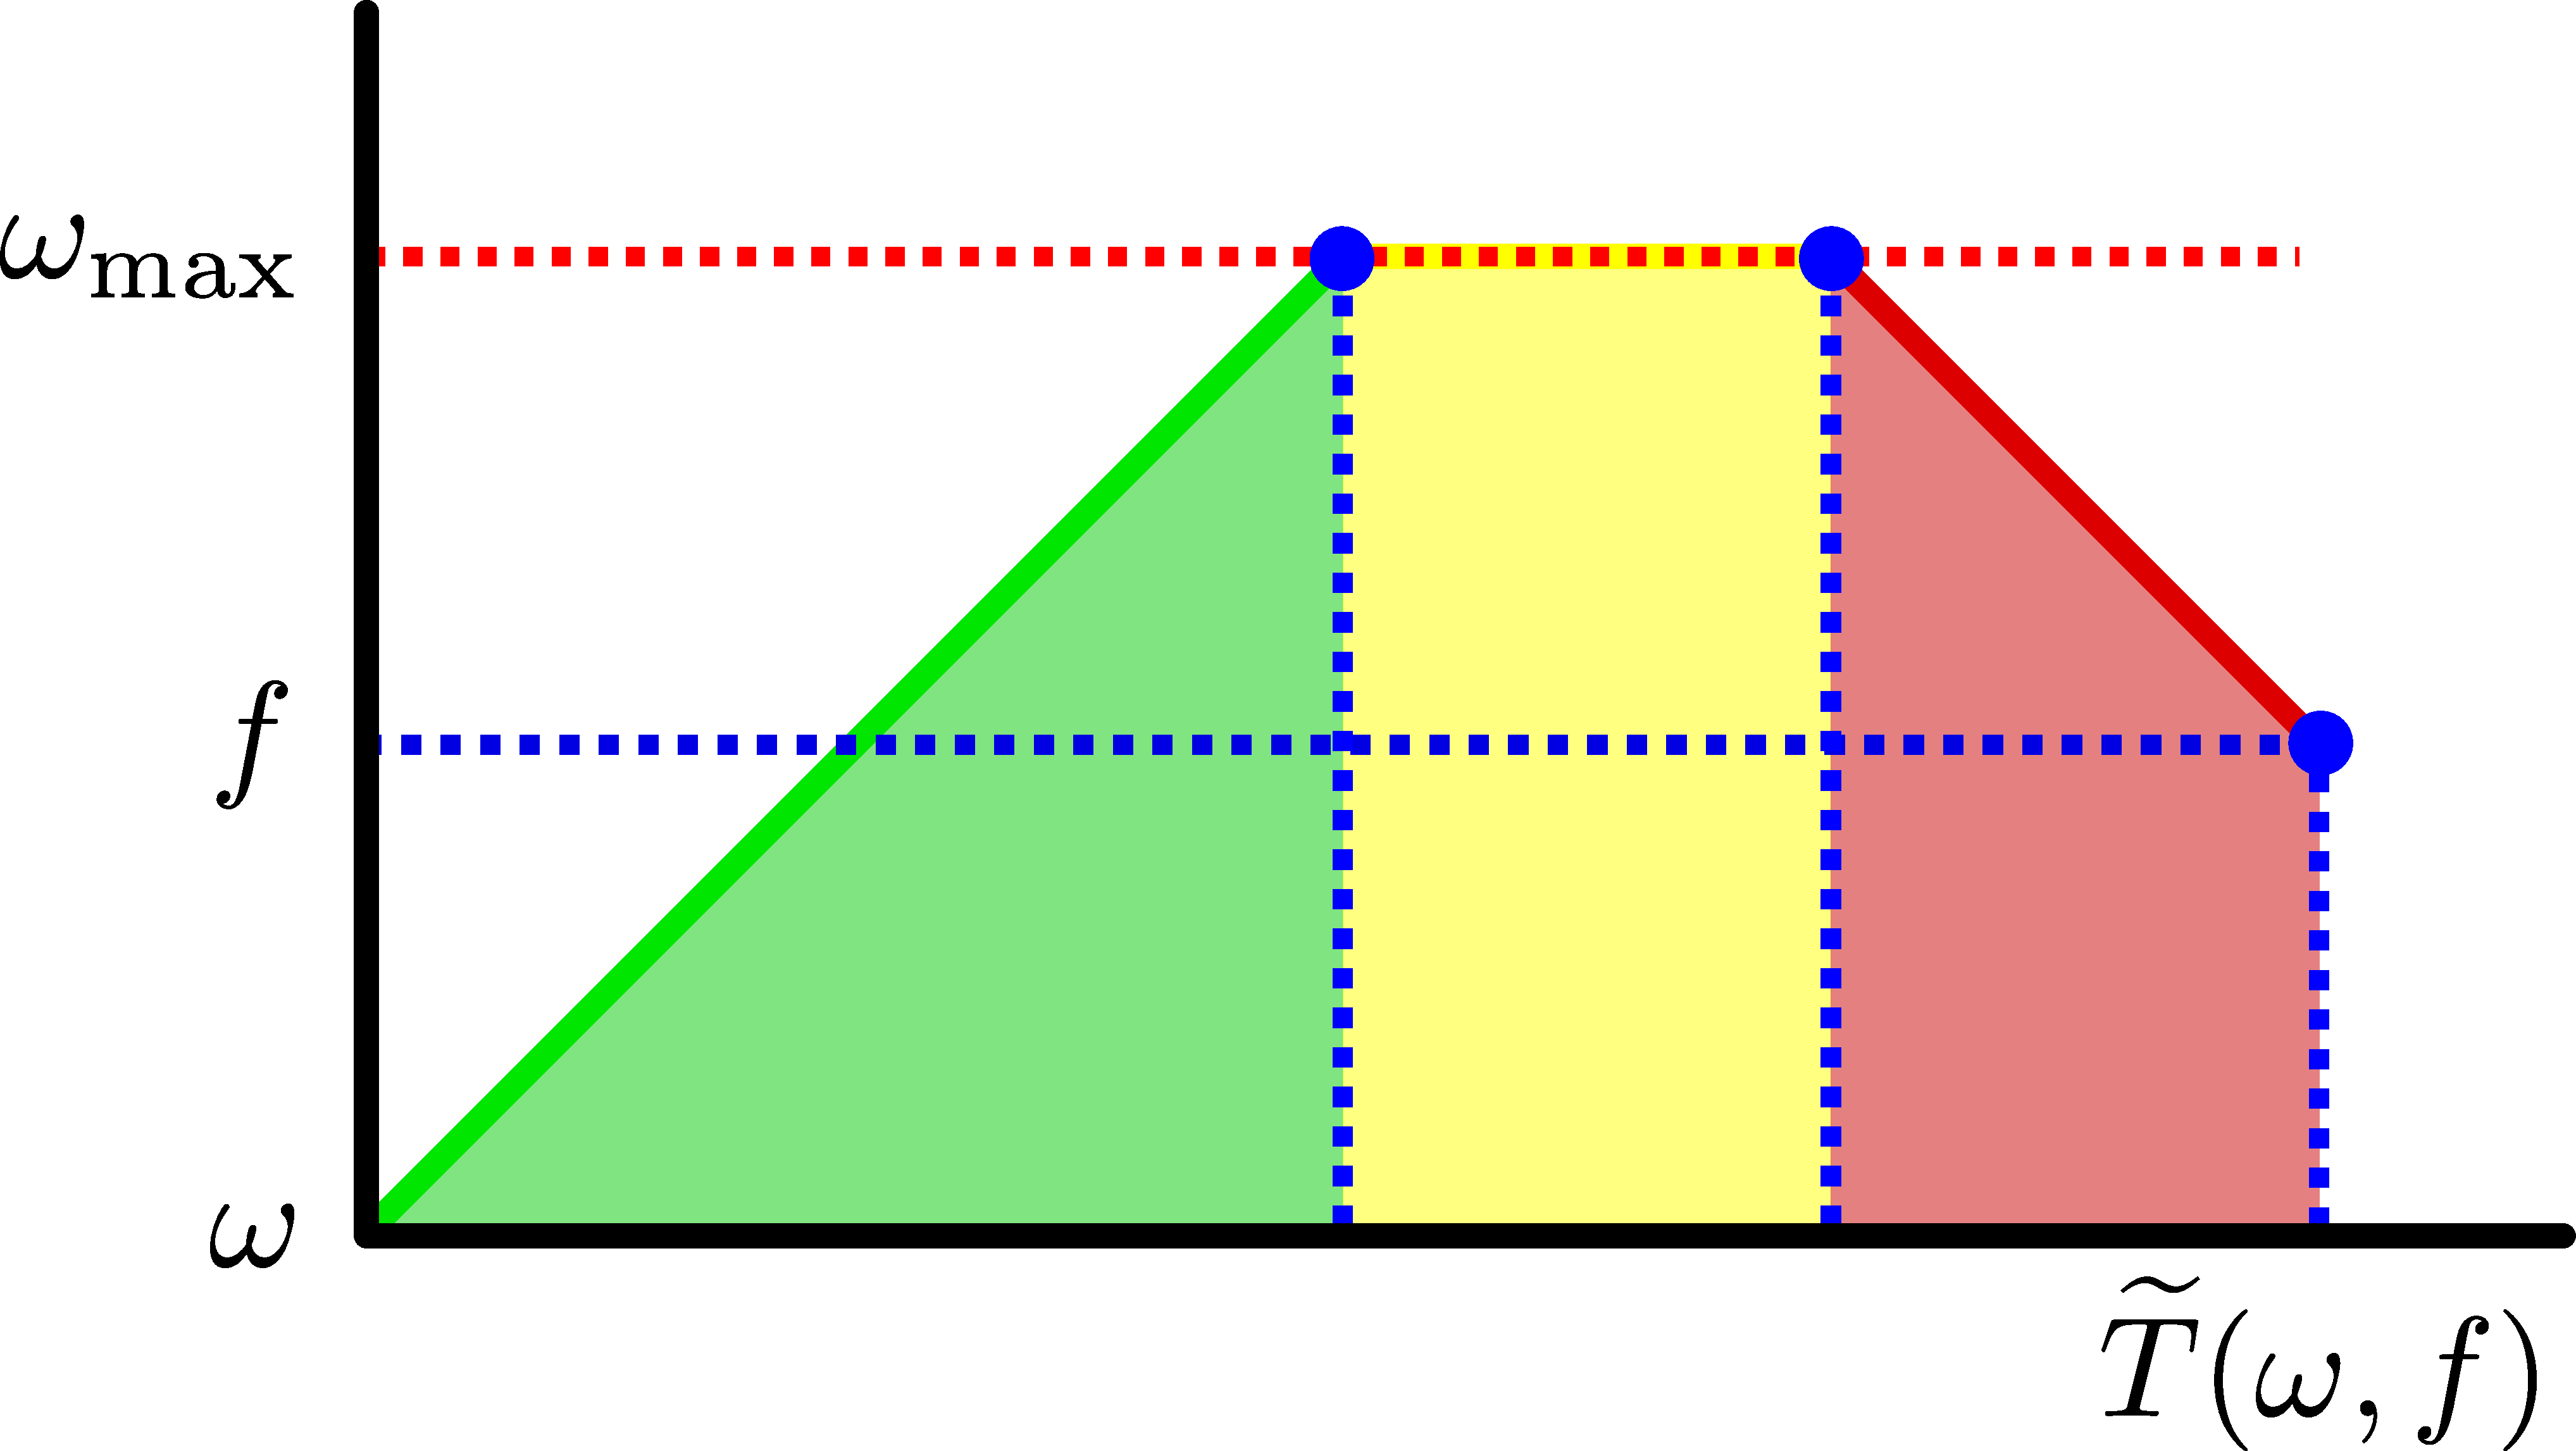
\includegraphics[scale=0.055]{Figures/mint-limitBare.pdf}}
      \label{fig:mintMax}
  \label{mintMax}
%\caption{Minimum interarrival time $\widetilde{T}(\omega,f)$ between speeds $\omega$ and $f$ where (a) $\omega_p(\omega,f) \leq \omega_{\max}$ and (b) $\omega_p(\omega,f) > \omega_{\max}$. Green, ascending lines represent periods of maximum acceleration, $\alpha_{\max}$, yellow, flat lines represent periods of zero acceleration, $\alpha = 0$, and red, descending lines represent periods of maximum deceleration, $\alpha_{\min}$.}
\caption{Minimum interarrival time $\widetilde{T}(\omega,f)$ between speeds $\omega$ and $f$ where (a) $\omega_p(\omega,f) \leq \omega_{\max}$ and (b) $\omega_p(\omega,f) > \omega_{\max}$.
Ascending, flat, and descending lines represent periods of maximum ($\alpha_{\max}$), zero, and  minimum ($\alpha_{\min}$) acceleration, respectively.}
\label{fig:mint}
\end{figure}

\begin{property}[Reversability of Inter-Arrival Times]
\label{T-reversal}
$\widetilde{T}(\omega(t_1),\omega(t_2)) = \widetilde{T}(\omega(t_2),\omega(t_1))$.
In other words, the minimum inter-arrival time from a job released at $\omega(t_1)$ to a job released at $\omega(t_2)$ is equal to the inter-arrival time when the speeds are in the reverse order.
\end{property} 


\paragraph{AVR Task Demand}
Let $\mathbb{W}$ be the set of all possible speed functions $\omega(t)$ that are feasible (i.e., $\omega(t)$ is any continuous function with acceleration between $\alpha_{\min}$ and $\alpha_{\max}$ and speeds between $\omega_{\min}$ and $\omega_{\max}$).
 For any such $\omega(t)$, considering that a computational job of an AVR task is released at time $t'$, we assume that the processor must successfully complete execution of this job by time $t' + \widetilde{T}(\omega(t'), \min(\Omega_1(\omega(t'), \alpha_{\max}),\omega_{max}))$; that is, the absolute deadline of this job coincides with the minimum time to complete a single rotation from a given speed $\omega(t')$. 
% \aaron{Is this deadline assumption problematic? We claim to use implicit deadline but the above implies that any non-maximally accelerated task would be constrained deadline. Thoughts?} 
We refer to an AVR task that sets deadlines in this way as a {\bf minimum angular deadline AVR task}~\cite{biondi_modeling_2018} and refer to the relative deadline of a job released at speed $\omega$ as 
%{\bf minimum relative deadline}, 
$\tilde{d}(\omega) = \widetilde{T}(\omega(t'), \min(\Omega_1(\omega(t'), \alpha_{\max}),\omega_{max}))$.
We may denote the {\em demand} of $\omega(t)$ over any $\delta$-length interval $[t_a, t_b]$ as $D_{\omega(t)}(t_a, t_b)$.
 $D_{\omega(t)}(t_a, t_b)$ represents the total execution requirement of jobs released by the speed function with both arrival times and absolute deadline in the interval $[t_a, t_b]$.
 More formally, if $\{t_1, t_2, \ldots\}$ is the set of times (in order) where the crankshaft triggers job releases following the speed function $\omega(t)$, then:
\begin{equation}
\label{eqn:d}
    D_{\omega(t)}(t_a, t_b) = \hspace{-.2in}\sum_{i: (t_i \geq t_a) 
            \wedge (t_i +\tilde{d}(\omega(t_i)) \leq t_b)}   \hspace{-.2in} c(\omega(t_i)).
\end{equation}

\noindent We can compute the upper envelope on the demand over any interval of length $\delta > 0$ for $\omega(t)$ as:
\begin{equation}\label{eqn:speed-fn-dbf}
    \dbf_{\omega(t)}(\delta) = \max_{t' \geq 0} \{D_{\omega(t)}(t', t' + \delta)\}.
\end{equation}

\noindent The \emph{worst-case demand} of an AVR task over any $\delta$-length interval is the speed schedule that maximizes the value of the upper envelope given in Equation~\ref{eqn:speed-fn-dbf}:
\begin{equation}\label{eqn:AVR-dbf}
    \dbf(\delta) = \max_{\omega(t) \in \mathbb{W}} \{\dbf_{\omega(t)}(\delta)\}.
\end{equation}
Considering any speed function $\omega(t)$ with job releases at speeds/times $\omega(t_1),\omega(t_2),\ldots$ in some interval $[t_a, t_b]$, it is clear that if we modify the function so that the crankshaft traverses one rotation in the minimum time (by Equation~\ref{eq:minTime}), then this will only lead to demand that exceeds or equals the original demand of $\omega(t)$.
Therefore, without loss of generality, we can restrict $\mathbb{W}$ to speed functions that traverse the rotation between job releases in the minimum possible time.
 This is essentially the observation made by Mohaqeqi et al.~\cite{mohaqeqi_refinement_2017} to reduce the problem of finding the worst-case $\omega(t) \in \mathbb{W}$ to the problem of identifying \emph{sequences of job release speeds}; i.e., the speed of the job releases entirely characterizes the speed function.
That is, we can completely describe any speed function $\omega(t)$ with job releases at times $t_1, t_2, \ldots$ instead by a sequence of speeds $(\omega_1 = \omega(t_1), \omega_2 = \omega(t_2), \ldots)$.
 Thus, after this point, we drop the speed-time function $\omega(t)$ and focus only on sequences of speeds.

\noindent The objective of this paper is to find an efficient way to calculate the worst-case AVR task demand defined in Equation~\ref{eqn:AVR-dbf}.

\begin{definition}[Reachable Speeds]\label{def:reachable-speeds}
Consider two speeds $\omega_1$ and $\omega_2$ such that $\omega_2\geq\omega_1$.
$\omega_2$ is said to be \emph{reachable} from $\omega_1$ if $\Omega_1(\omega_1,\alpha_{max})\geq \omega_2$.
\end{definition}

\begin{definition}[Valid Sequence]\label{def:valid-sequence}
A set of jobs ${j_1,j_2,j_3,\ldots,j_k}$ released at speeds $\omega_1,\omega_2,\ldots,\omega_k$ is said to be a valid sequence of speeds if 
%Original footnote
%$\forall i \in \mathbb{N}^k_2\footnote{$\mathbb{N}^k_j$ represents the set $\{j,j+1,\ldots,k\}$},\,\omega_i$ is reachable from $\omega_{i-1}$.
$\forall i \in \mathbb{N}^k_2$, $\omega_i$ is reachable from $\omega_{i-1}$ where $\mathbb{N}^k_j$ is the set of natural numbers from \textit{j} to \textit{k}, i.e., $\{j,j+1,\ldots,k\}$.
%$\forall i \in \{2,\ldots,n\},\, \Omega(\omega(t_i),\alpha_{min}))\geq \omega(t_{\mathit{i-1}})$ and $\forall i \in \{1,\ldots,n-1\},\, \Omega(\omega(t_i),\alpha_{max}))\leq \omega(t_{\mathit{i+1}})$. 
%and $\Omega(\omega(t_2),\alpha_{min})\geq\omega(t_1)$ 
\end{definition}
\paragraph{Problem Definition} 
%Potentially there can be infinite sequences of jobs released depending on the instantaneous angular speed and angular acceleration of the crankshaft. 
Consider a minimum angular deadline AVR task, which is characterized by feasible speed $\left[\omega_{\min}, \omega_{\max}\right]$ and acceleration $\left[\alpha_{min}, \alpha_{max}\right]$ ranges, where $\alpha_{max} = |\alpha_{min}|$, and a set of modes $\mathbf{\Omega_{rb}}=\{\omega_{rb_1}, \ldots, \omega_{rb_m} \}$, each of which is associated with an execution time $c(\omega_{rb_i})$, $i = 1, \ldots, m$, as discussed earlier in this section.
The objective is to find $\dbf(\delta)$ (Equation~\ref{eqn:AVR-dbf}), the worst-case demand of the AVR task over any $\delta$-length interval $[t_a, t_b]$ assuming that the acceleration of the crankshaft may change within a single rotation.

\subsection{Knapsack-based approach for deriving the worst-case demand}
\label{sec:knapsack}

We now describe the problem transformation from calculating $\dbf(\delta)$ to a variant of the knapsack problem.
This section both provides context for and relies upon several  properties and  lemmas defined in Sections \ref{sec:filterSeq} and \ref{sec:Summary}.
Briefly, \textit{dominant speed sequences} are sequences of job release speeds whose demand %is equivalent to the maximum demand of a task over a given interval length (i.e., the demand of a dominant speed sequence 
coincides with the value of Equation \ref{eqn:AVR-dbf}.
These dominant speed sequences are non-decreasing (see Section \ref{subsec:seq-transform}, Lemma \ref{lemma:non-decreasing}) and start at right boundary speeds (see Section \ref{sec:dominant-start}, Lemma \ref{lemma:startSpeed}).

% {\color{blue}Add a paragraph outlining what to expect later. Aaron: Is the above sufficient?}
% \sandeep{I think we will need to explain about the items in the knapsack too. In the 2nd and 3rd paragraphs from here, we explain about the dependency of the items in the knapsack. I think this will be challenging to do without actually giving the proofs.}
% \aaron{I believe this is already done. See paragraph immediately following.}
% \sandeep{We do not explain about the limited numbers of jobs following a given job and about the sequence only being non-decreasing. One way to do this is just note all the constraints on the sequences we prove later and say that for proof please refer to later sections.}

In the traditional knapsack problem, the aim is to maximize the total profit from a given set of items where each item is associated with a profit and weight, while ensuring that the aggregate weight is less than or equal to the maximum allowable weight of the knapsack.
Our goal is to transform the problem of finding $\dbf(\delta)$ into a variant of the knapsack problem.
In our case, a job is equivalent to an item.
%and is characterized by: the speed at the beginning of the rotation, the corresponding execution time, and the minimum inter-arrival time given the speed at the beginning of the rotation (Equation~\ref{eq:minTime}) -- which depends on the initial speed of the subsequent job.
As such, the ``weight" of a job (i.e., item) is the minimum inter-arrival time, and the ``profit" is its execution time.
The goal, then, is to maximize demand (i.e., profit) over a time interval ($\delta$).

Since a dominant speed sequence is non-decreasing (Lemma~\ref{lemma:non-decreasing}), a job's execution time may contribute to the demand bound function $\dbf(\delta)$ more than once.
As such, our knapsack problem is, in fact, a bounded knapsack problem.
In addition, since  adjacent speeds in a dominant speed sequence must be reachable from one another (Definition \ref{def:reachable-speeds}), once an item, i.e., job, has been included in the knapsack, there is a finite number of jobs that can follow, making our problem a bounded precedence constraint knapsack problem (BPCKP)~\cite{cho_depth-first_1997,johnson_knapsacks_1983}.
Fig.~\ref{fig:Knapsack1} provides a visual example representation of our problem as a BPCKP.
For clarity, the subscripts of the speeds are used to denote the precedence constraints.
\begin{figure}
\centering
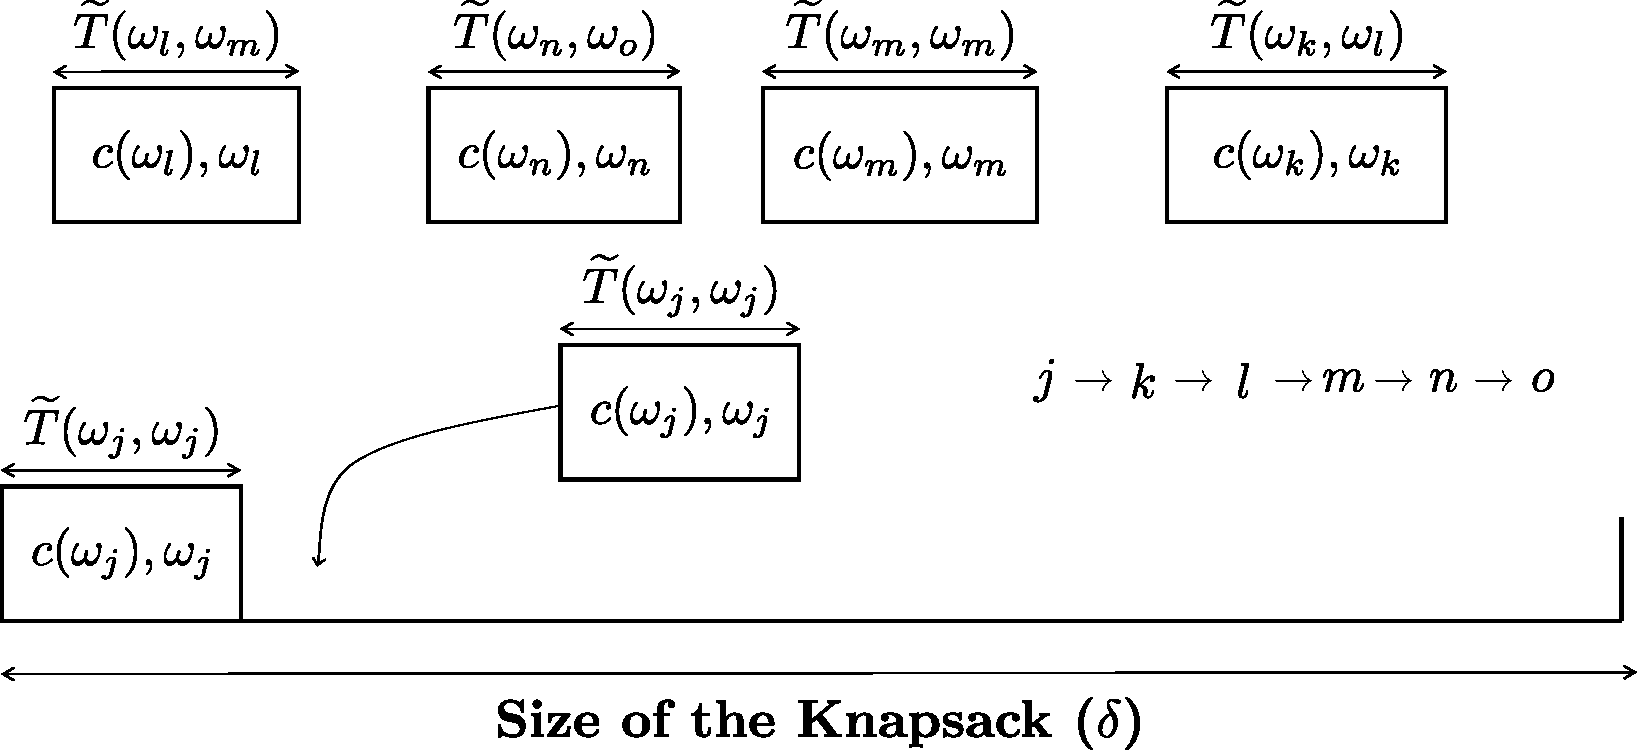
\includegraphics[width=1.0\linewidth]{Figures/vectorKnapsackv2.pdf}
\caption{Example items for our knapsack problem. A job that is higher in the precedence relation is preceded by a job lower in the relation.}
\label{fig:Knapsack1}
\end{figure}

%PNG
%\begin{figure}
%\centering
%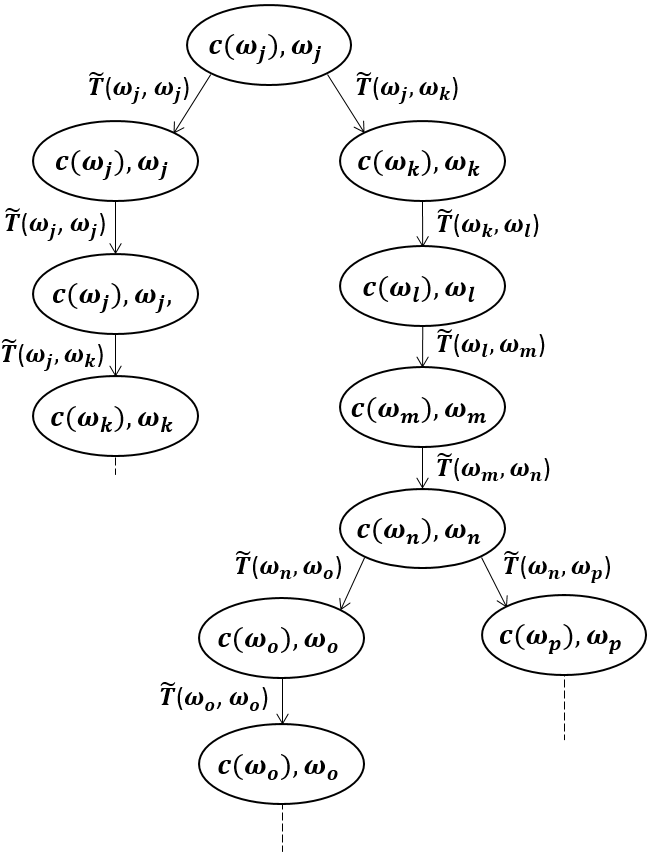
\includegraphics[width=0.5\linewidth]{Figures/KnapsackTree.PNG}
%\caption{Precedence constraints among jobs are expressed using out-trees.}
%\label{fig:KnapsackTree}
%\end{figure}

%Vectorized Image
%\begin{figure}
%    \centering
%    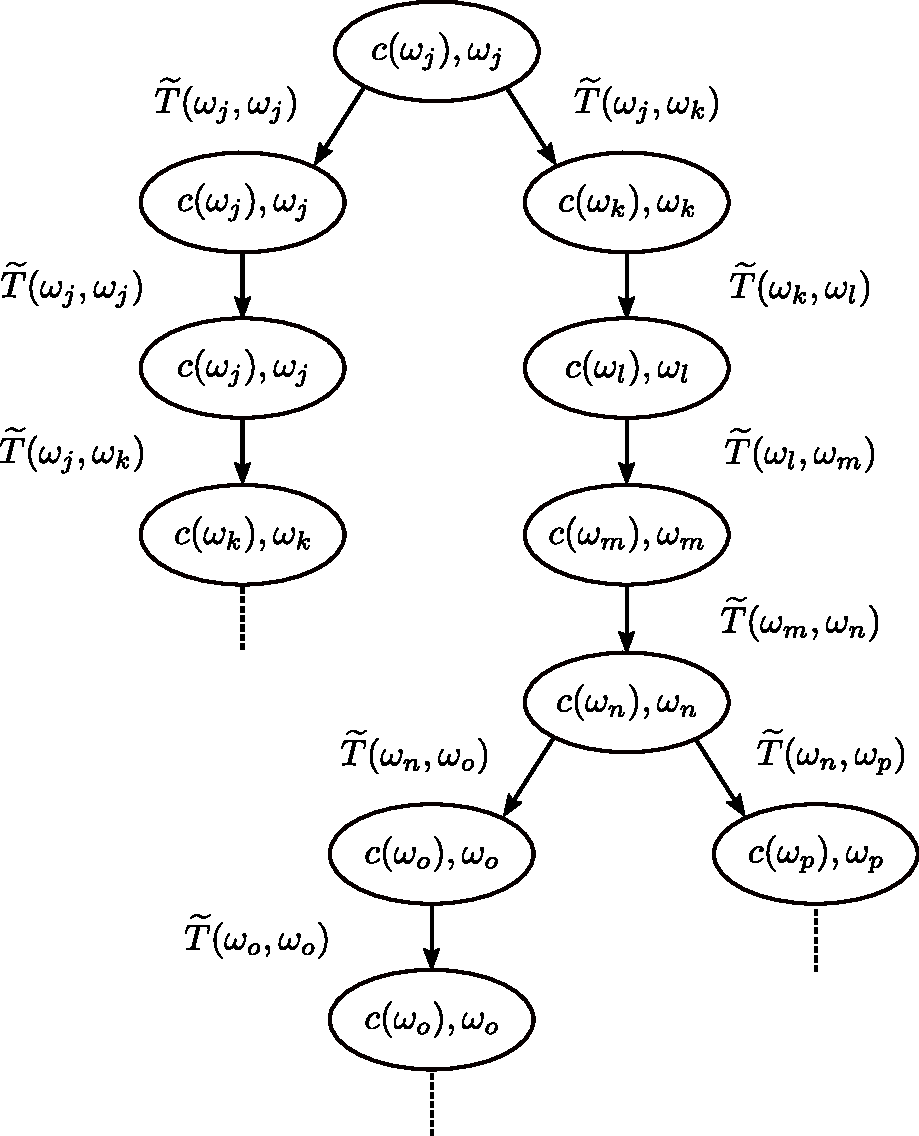
\includegraphics[width=0.8\linewidth]{Figures/vectorKnapsackTreeIsolated.pdf}
%    \caption{Precedence constraints among jobs are expressed using out-trees.}
%    \label{fig:KnapsackTree}
%\end{figure}

%Vectorized, Shortened
\begin{figure}
    \centering
    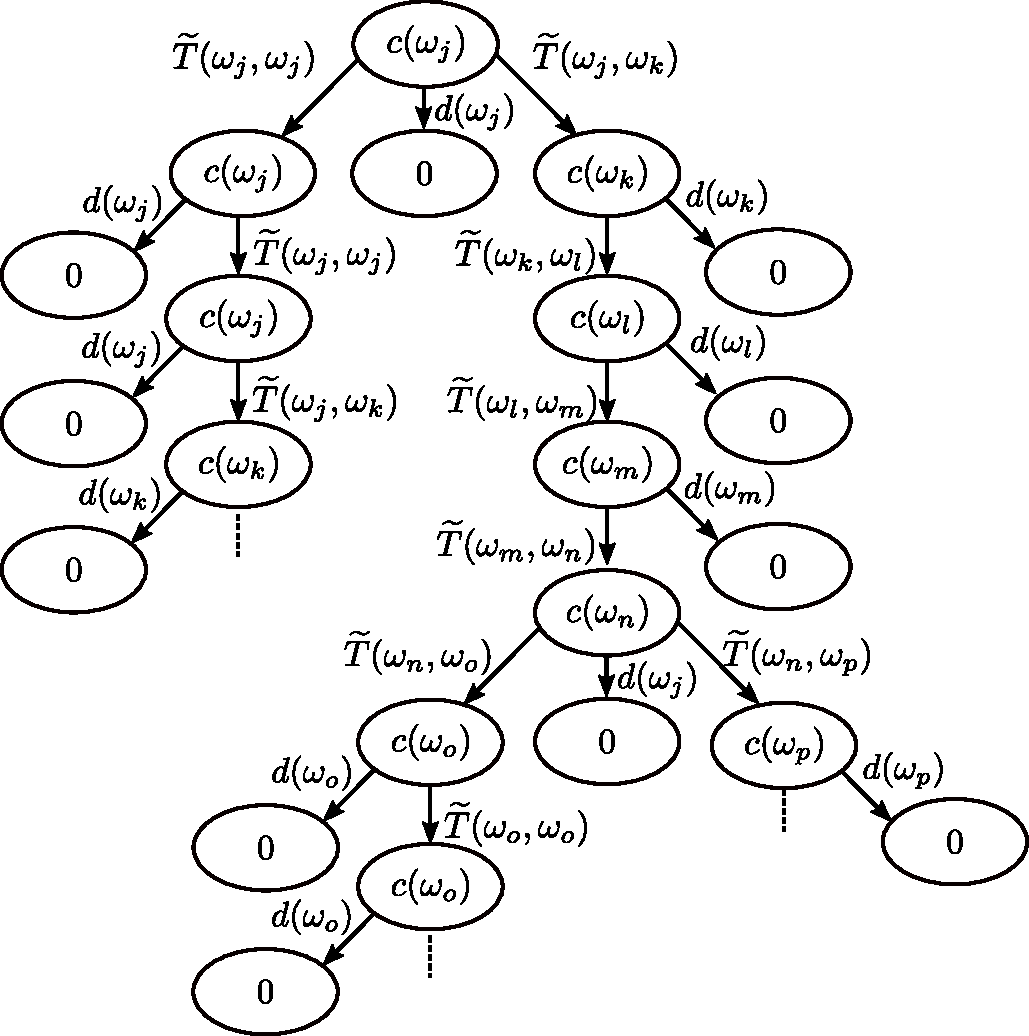
\includegraphics[width=1.0\linewidth]{Figures/vectorKnapsackTreeShortenedv5.pdf}
    \caption{Precedence constraints among jobs are expressed using out-trees. Nodes represent WCETs for the initial speeds and arrows represent minimum inter-arrival times. The tree demonstrates the various precedence relations and possible paths. Leaves represent completion of the parent job without adding subsequent jobs (i.e. items). Furthermore, each of the leaves has zero execution since its parent is the final job included in the knapsack.}
    \label{fig:KnapsackTree}
\end{figure}

An effective way to model the precedence constraints among jobs is by using out-trees.
The sequences beginning at each of the source nodes are independent of each other (i.e., sequences beginning at each of the right boundary speeds according to Lemma~\ref{lemma:startSpeed}).
An example out-tree is shown in Fig. \ref{fig:KnapsackTree}.
To represent the trees in a knapsack problem, we define a dependency graph $G_I=(V_I, A_I)$, where $V_I$ denotes the set of vertices (i.e., items) in the out-tree $G_I$~\cite{kellerer_knapsack_2004}.
An edge between any two vertices denotes that the two speeds are reachable from one another and is represented by $(j,k)\in A_I$.
Formally, our BPCKP can be expressed as follows:
\begin{alignat}{3}
    & \underset{x}{\text{maximize}}
    & \quad & \sum_{j}\sum_{r=1}^{M_\delta} c(\omega_j) \cdot x_j^{r} \label{eqn:maxDemand}\\
    & \text{subject to}
    & \quad & \sum_{j, k | (j,k) \in A_I} \sum_{r=1}^{M_\delta}  \tilde{T}(w_j, w_k) \cdot x_k^r \leq \delta \label{eqn:kp-cons}\\
    & & \quad & \sum_{k|(j,k)\in A_I} x_k^1 \leq 1, \, \forall j \label{eqn:singleKnapsackPath}\\
    & & \quad & x_j^1 \geq x_k^1, \, \forall (j,k)\in A_I \label{eqn:precedenceConstraint}\\
    %& & \quad & m \in \{1,2,3,...,M_\delta\} %\label{eqn:mValueSet}\\
    % & & \quad & M = 1,2,.. \,\,\forall \omega_j \in \mathbf{\Omega_{rb}}\\
    % & & \quad & x_j^{\eta_j} \geq x_k^{\eta_k}, \,\, (j,k)\in A_I \label{eqn:kp-prec}\\
    %& & \quad & x_j^{m} \in \{0,1\} \\
    & & \quad & x_j^r \geq x_j^{r+1}, \,\, \forall j, r \in \{1,2,3,...,M_\delta-1\} \label{eqn:multipleJobRestriction}\\
     & & \quad &x_j^r \in \{0,1\},\,\forall j,  r \in \{1,2,3,...,M_\delta\} \label{eqn:binaryXValue}
    % & & \quad & \eta_j \in \mathbb{Z}^+ \,\, \forall \, x_j^{\eta_j} \, | \, \omega_j \in \mathbf{\Omega_{rb}} \label{eqn:eta-boundary-jobs}\\
    % & & \quad & \eta_j \in \{0,1\} \,\, \forall \, x_j^{\eta_j} \, | \, \omega_j \notin \mathbf{\Omega_{rb}} \label{eqn:eta-special-jobs}
\end{alignat}
%Original Eqn:
% \noindent maximize
% \begin{equation}
% \sum_{j=1}^{\infty}c(\omega_j) \cdot x_j^\eta
% \end{equation}
% \newline
% subject to
% \begin{equation}
% \label{eqn:kp-cons}
% \sum_{j=1}^{\infty}\widetilde{T}(\omega_j, \omega_k) \cdot x_j^\eta \leq \delta
% \end{equation}
% \begin{equation}\label{eq:kp3}
% x_j^\eta \geq x_k^\eta, \,\, (j,k)\epsilon A_I
% \end{equation}
\noindent where $M_\delta$ represents an upper bound on the number of job releases in a $\delta$-length interval and  $x_j^r$ is a binary variable: $x_j^r$ is one if there are at least $r$ jobs released at speed $\omega_j$ in the knapsack; otherwise, $x_j^r$ is zero.
Equation \ref{eqn:maxDemand}  maximizes total demand.
Equation \ref{eqn:kp-cons} requires all deadlines of selected jobs fall within the $\delta$-length interval.
Equation \ref{eqn:singleKnapsackPath} permits at most one child node of each parent node to be added to the knapsack.
Equation \ref{eqn:precedenceConstraint} enforces the precedence constraint such that no child node may be added without its parent.
Equation \ref{eqn:multipleJobRestriction} ensures repeated jobs of a particular speed $\omega_j$ are added incrementally to (and do not skip indices of) $x_j^r$ (i.e, if $x_j^\ell = 0$, then for all $s > \ell: x_j^s = 0$). 

%Original Paragraph (20180928)
% Original Paragraph (20180928):
% where, $x_j^{\eta_j}$ denotes the $\eta_j^{th}$ job released at speed $\omega_j$. It is worth noting that Equation \ref{eqn:eta-boundary-jobs} allows unlimited job releases at right boundary speeds while Equation \ref{eqn:eta-special-jobs} allows at most one job release from non-right-boundary speeds. In Equation~\ref{eqn:kp-cons}, $\omega_j$ and $\omega_k$ denote the speeds at the beginning and the end of a rotation, respectively. Equation~\ref{eqn:kp-prec} requires that $\forall (j,k)\in A_I$, at least one job must be released at $\omega_j$ before a subsequent job is released at $\omega_k$. Since the sub-solutions of a BPCKP have been shown to have optimal substructures, a BPCKP can be solved recursively.

% \subsection{Algorithm}
%{\color{blue}Placed the algorithm below knapsack based on Friday's meeting.}
Algorithm~\ref{algo} shows our pseudocode for the dynamic programming approach to solve the bounded precedence constraint knapsack problem.
The \emph{CalculateDemand} function is initially called with the parameters $\omega \in \mathbf{\Omega_{rb}}$ and $\delta$, the total time length.
The \emph{maxDemand} parameter keeps track of the highest demand computed until the current instance of the recursive loop.
In each recursive instance, the next speed is chosen from the list of %the speeds possible for the next job release
possible next job release speeds according to Theorem~\ref{thm:dominant-set} (Section \ref{sec:Summary}).
The variable $D_w$ (Equation~\ref{eqn:d}) tracks the accumulated demand of the current sequence.


\begin{algorithm}
\begin{algorithmic}[1]
\Function {CalculateDemand}{$\omega$,$\delta$}:
\State maxDemand $\gets 0$
\\
\If {StoredDemand($\omega,t)\neq\phi$}
\State return StoredDemand($\omega$,$\delta$)
\EndIf    
\\
\If	{$\delta < \Tilde{d}(\omega)$}
\State return 0
\EndIf
\\
\For {$\omega'$ in $\sf{nextPossibleSpeed}(\omega)$} \Comment{See Theorem~\ref{thm:dominant-set}}
\State $\delta \gets \delta-\widetilde{T}(\omega,\omega')$
\State $D_w \gets c(\omega) +$ CalculateDemand($\omega'$,$\delta$)\\
\If {$D_w >$ maxDemand}
\State maxDemand $\gets D_w$
\EndIf
\EndFor
\\
\State StoredDemand($\omega$,$\delta$) $\gets$ maxDemand
\State return maxDemand
\EndFunction
\end{algorithmic}
\caption{DP for Calculating $\dbf(\delta)$}
\label{algo}
\end{algorithm}

\subsection{Dominant Speed Sequences}
\label{sec:filterSeq}
The previous section outlined how dominant speed sequences facilitate the problem transformation from calculating $\dbf(\delta)$ to a variant of the knapsack problem.
This section formally defines Lemma \ref{lemma:non-decreasing} and Lemma \ref{lemma:startSpeed}
%, and Theorem \ref{thm:dominant-set} 
referenced in the above BPCKP approach.

The main challenge in determining the worst-case demand of an AVR task is the variation in the execution time, which varies as a function of the angular speed. 
Earlier work, e.g., Mohaqeqi et al.~\cite{mohaqeqi_refinement_2017} showed that the speed sequences that maximize demand contain only speeds from some finite set.
 Mohaqeqi et al. used this set to design a DRT task which considers all possible feasible sequences of speeds.
 However, this can still lead to a large number of speed permutations to check when searching for the worst-case demand.
 As mentioned in the related work section, we show that we can greatly limit the sequences that need to be considered in the \emph{dominant speed sequence set} when we consider minimum angular deadline AVR tasks with $\alpha_{max} = |\alpha_{min}|$.
  A \emph{dominant speed sequence} is  a speed sequence whose demand is equivalent to the maximum demand of a task over a given interval length (i.e., its demand coincides with the value of Equation~\ref{eqn:AVR-dbf}).
 A \textit{dominant speed sequence set} is a set of speed sequences that must contain the dominant speed sequence.
In this section, we derive the necessary characteristics of a dominant speed sequence.
\vspace{-1mm}
\paragraph{Properties of Minimum Inter-arrival Times and Deadlines}\label{subsec:min-arrival-times}

We begin by establishing some useful properties regarding the minimum inter-arrival time function $\widetilde{T}(\omega, f)$ (Equation~\ref{eq:minTime}) that will be used to prove some characteristics of dominant speed sequences.
 The first property is that $\widetilde{T}(\omega, f)$ is always positive, which was already proved in previous work on AVR tasks~\cite{mohaqeqi_refinement_2017}.
We abuse terminology and refer to some lemmas as properties to make supporting concepts easier to read.

\begin{property}[Positive Minimum Inter-arrival Times] \label{prop:pos-min-interarrival}
For all $\omega, f \in [\omega_{\min}, \omega_{\max}]$,
\begin{equation}\label{eqn:pos-min-interarrival}
    \widetilde{T}(\omega, f) > 0.
\end{equation}
\end{property}

%%%NWF: I don't think this proof is necessary.
%%%%%%%%%%%%%%%%%BEGIN COMMENT%%%%%%%%%%%%%%%%%%%%%%%%%%%%%%%%%%%%%%%%
\begin{comment}
%\fishern{Aaron-- please insert your statements and proof here}
\subsubsection{Minimum Interarrival Time Properties}
We first establish some mathematical properties regarding $\widetilde{T}$ (Equation \ref{eq:minTime}):
\subparagraph{Nonnegative Interarrival Times} In the case where $\omega_p(\omega,f) \leq \omega_{\max}$, $\sqrt{2\omega^2+2f^2+4\alpha_{\max}} > \omega + f$ thus the interarrival time is always positive. In the case where $\omega_p(\omega,f) > \omega_{\max}$, the following inequality demonstrates nonnegative interarrival time as well:
\begin{alignat}{3}\label{eq:minimumTimeNonNegative}
&& \omega_p(\omega,f) & > \omega_{\max}& \nonumber \\
\Leftrightarrow && \frac{\sqrt{2\omega^2+2f^2 + 4\alpha_{\max}}}{2} & > \omega_{\max} \nonumber \\
\Leftrightarrow && 2\omega^2+2f^2 + 4\alpha_{\max} - 4\omega_{\max}^2\alpha_{\max} & > 0 \nonumber \\
\Leftrightarrow && \frac{2\omega^2+2f^2 + 4\alpha_{\max}}{4\omega_{\max}\alpha_{\max}} - \frac{4\omega_{\max}^2\alpha_{\max}}{4\omega_{\max}}& > 0 \nonumber \\
\Leftrightarrow && \frac{2\omega^2+2f^2 + 4\alpha_{\max}}{4\omega_{\max}\alpha_{\max}} - \frac{4\omega_{\max}^2\alpha_{\max}}{4\omega_{\max}}& > 0 \nonumber \\
\Leftrightarrow && \frac{2\omega^2+2f^2 + 4\alpha_{\max}}{4\omega_{\max}\alpha_{\max}} - \frac{4\omega_{\max}^2\alpha_{\max}}{4\omega_{\max}}& > 0 \nonumber \\
\Leftrightarrow && \frac{\omega^2+f^2}{2\omega_{\max}\alpha_{\max}} - \frac{2\omega_{\max}^2\alpha_{\max}}{2\omega_{\max}\alpha_{\max}} + \frac{2\alpha_{\max}}{2\omega_{\max}\alpha_{\max}}& > 0 \nonumber \\
\Leftrightarrow && \frac{2\omega_{\max} -\omega -f}{\alpha_{\max}} + \frac{\omega^2+f^2}{2\omega_{\max}\alpha_{\max}} - \frac{\omega_{\max}}{\alpha_{\max}} + \frac{}{\omega_{\max}}& > 0 \nonumber \\
\Leftrightarrow && \frac{\omega_{\max} -\omega -f}{\alpha_{\max}} + \frac{\omega^2+f^2}{2\omega_{\max}\alpha_{\max}} + \frac{}{\omega_{\max}}& > 0 \nonumber \\
\Leftrightarrow && \widetilde{T}(\omega,f) & > 0
\end{alignat}
\end{comment}
%%%%%%%%%%%%%%%%%END COMMENT%%%%%%%%%%%%%%%%%%%%%%%%%%%%%%%%%%%%%%%%
We next show that $\widetilde{T}(\omega, f)$ is always non-increasing as we increase either the starting speed $\omega$ or the ending speed $f$.

\begin{property}[Minimum Inter-arrival Time Decreases with  Starting/Ending Speeds] \label{prop:neg-deriv-min-interarrival}
For all $\omega, f \in [\omega_{\min}, \omega_{\max}]$,
\begin{equation}\label{eqn:neg-deriv-min-interarrival}
\frac{\partial \widetilde{T}(\omega,f)}{\partial \omega} \leq 0~~~~ \textrm{and} ~~~~\frac{\partial \widetilde{T}(\omega,f)}{\partial f} \leq 0.
\end{equation}
\end{property}
\begin{proof}
Observe that the partial derivative of $\widetilde{T}$ with respect to $\omega$ and $f$, respectively are:
\begin{equation} \label{eq:minTimeDerivativeWrtInitial}
\frac{\partial \widetilde{T}(\omega,f)}{\partial \omega} =
\left\{
    \begin{array}{ll}
        \frac{\frac{2\omega}{\sqrt{4\alpha_{\max}+2f^2+2\omega^2}}-1}{\alpha_{\max}} & {\rm if}~ \omega_p(w,f) \leq \omega_{\max} \ \\
        \frac{\omega}{\omega_{\max}\alpha_{\max}} -\frac{1}{\alpha_{\max}}  & {\rm if}~ \omega_p(w,f) > \omega_{\max}
    \end{array}
\right.
\end{equation}
%\noindent and
\begin{equation} \label{eq:minTimeDerivativeWrtFinal}
\frac{\partial \widetilde{T}(\omega,f)}{\partial f} =
\left\{
    \begin{array}{ll}
        \frac{\frac{2f}{\sqrt{4\alpha_{\max}+2f^2+2\omega^2}}-1}{\alpha_{\max}} & \omega_p(w,f) \leq \omega_{\max} \ \\
        \frac{f}{\omega_{\max}\alpha_{\max}} - \frac{1}{\alpha_{\max}}  & \omega_p(w,f) > \omega_{\max}
    \end{array}
\right.
\end{equation}
The above partial derivatives are clearly always non-positive for any $\omega, f \in [\omega_{\min}, \omega_{\max}]$.
\end{proof}

We now focus upon the relative deadline of a job released at speed $\omega$  (i.e., $\Tilde{d}(\omega))$.
 We can show that the relative deadline decreases as we increase the speed the job is released at.
 Furthermore, the rate of decrease for the relative deadline of a job is faster than the rate of decrease in the minimum inter-arrival time of the next job.

\begin{property}[Rate of Change of Relative Deadline] \label{prop:deadline-derivative}
For all $\omega, f \in [\omega_{\min}, \omega_{\max}]$ where $f$ is reachable from $\omega$:
\begin{equation}\label{eqn:deadline-derivative}
\frac{\partial \Tilde{d}(\omega)}{\partial \omega}< 0~~~~ \textrm{and} ~~~~\frac{\partial \Tilde{d}(\omega)}{\partial \omega} \leq \frac{\partial \widetilde{T}(\omega,f)}{\partial \omega}.
\end{equation}
\end{property}
\begin{proof}
First, consider the partial derivative of $\Tilde{d}(\omega)$, given below.
 It is clear from the expression that it is always negative for all $\omega \in [\omega_{\min}, \omega_{\max}]$.

% \begin{equation} \label{eq:minTimeFinalJobDerivative}
%     \frac{\partial \Tilde{d}(\omega)}{\partial \omega} = \frac{\frac{\omega}{\sqrt{\omega^2+2\alpha_{\max}}}-1}{\alpha_{\max}} < 0
% \end{equation}
\begin{equation}
\Tilde{d}(\omega) =
\left\{
    \def\arraystretch{1.5}
    \begin{array}{ll}
        \frac{\sqrt{\omega^2+2\alpha_{\max}}-\omega}{\alpha_{\max}} & \Tilde{d}_p(w) \leq \omega_{\max} \ \\
        -\frac{\omega}{\alpha_{\max}} + \frac{\omega^2 + \omega_{\max}^2}{2\omega_{\max}\alpha_{\max}}+\frac{1}{\omega_{\max}}  & \Tilde{d}_p(w) > \omega_{\max}
    \end{array}
\right.
\end{equation}
\begin{equation}
\Tilde{d}_p(\omega) = \sqrt{\omega^2 + 2\alpha_{\max}\, \theta}
\end{equation}
where $\Tilde{d}(\omega)$ is derived from Equation \ref{eqn:rotation} such that $\Tilde{d}(\omega) = \frac{\Omega_1(\omega,\alpha_{\max}) - \omega}{\alpha_{\max}}$ if $\Tilde{d}_p(w) \leq \omega_{\max}$ and $\Tilde{d}(\omega) = \widetilde{T}(\omega,\omega_{\max})$ if $\Tilde{d}_p(w) > \omega_{\max}$.
\begin{equation} \label{eq:minTimeFinalJobDerivative}
\frac{\partial  \Tilde{d}(\omega)}{\partial \omega} =
\left\{
    \def\arraystretch{1.5}
    \begin{array}{ll}
        \frac{\frac{\omega}{\sqrt{\omega^2+2\alpha_{\max}}}-1}{\alpha_{\max}} & \Tilde{d}_p(w,f) \leq \omega_{\max} \ \\
        \frac{\omega}{\omega_{\max}\alpha_{\max}} - \frac{1}{\alpha_{\max}}  & \Tilde{d}_p(w,f) > \omega_{\max}
    \end{array}
\right.
\end{equation}
where $\Tilde{d}$ is derived by replacing $f$ with Equation~\ref{eqn:rotation} in the definition of minimum angular deadline AVR task when $\Tilde{d}_p(w) < \omega_{\max}$.
By supposition, $f$ is reachable from $\omega$; thus by definition of reachable,
\begin{equation} \label{eq:partialEpartialwCompare}
\begin{array}{ll}
          { } & f  \leq  \Omega_1(\omega, \alpha_{\max})\nonumber\\
    \Leftrightarrow & f  \leq  \sqrt{\omega^2+2\alpha_{\max}} \nonumber \\
%f^2  \leq  \omega^2+2\alpha_{\max} \nonumber \\
    \Leftrightarrow &  2f^2  \leq  2\omega^2+4\alpha_{\max} \nonumber \\
    \Leftrightarrow &  4\alpha_{\max}+2f^2+2\omega^2  \leq  4\omega^2+8\alpha_{\max} \nonumber \\
    %\sqrt{4\alpha_{\max}+2f^2+2\omega^2}  \leq  2 \sqrt{\omega^2+2\alpha_{\max}} \nonumber \\
    \Leftrightarrow &   \omega \sqrt{4\alpha_{\max}+2f^2+2\omega^2}  \leq  2\omega \sqrt{\omega^2+2\alpha_{\max}} \nonumber \\
    %\frac{\omega}{\sqrt{\omega^2+2\alpha_{\max}}}  \leq  \frac{2\omega}{\sqrt{4\alpha_{\max}+2f^2+2\omega^2}} \nonumber \\
    \Leftrightarrow &   \frac{\frac{\omega}{\sqrt{\omega^2+2\alpha_{\max}}}-1}{\alpha_{\max}}  \leq  \frac{\frac{2\omega}{\sqrt{4\alpha_{\max}+2f^2+2\omega^2}}-1}{\alpha_{\max}} \nonumber \\
    \Leftrightarrow &  \frac{\partial \Tilde{d}(\omega)}{\partial \omega}  \leq  \frac{\partial \widetilde{T}(\omega,f)}{\partial \omega}
\end{array}
\end{equation}
\end{proof}

%\fishern{Making a pass from this point -- 12:43pm 5/31}
\paragraph{Speed Sequence Order Transformations}
\label{subsec:seq-transform}

In this subsection, we describe how given a valid speed sequence $S = (\omega_1, \omega_2, \ldots, \omega_n)$, we may transform it to one in non-decreasing order without reducing the total demand of the sequence.
 We begin with some notation that will be employed in describing the transformations.


\begin{definition}[Non-Decreasing Speed Sequence]\label{def:seq-ascending}
Given any valid, finite speed sequence $S = \{\omega_1, \omega_2, \ldots, \omega_n\}$, we define $S_A = (s_1, s_2, \ldots, s_n)$ to be the sequence obtained from reordering the speeds of $S$ in a non-decreasing order (i.e., $s_1$ is the smallest $\omega_i$ in $S$ and $s_n$ is the largest).
 We call $S_A$ a \emph{non-decreasing speed sequence} of $S$.
\end{definition}

We can show that for any valid sequence $S$ (in arbitrary speed order) the corresponding non-decreasing sequence $S_A$ must also be valid.

\begin{property}[Validity of Non-Decreasing Sequences]\label{prop:non-dec-valid}
If $S= (\omega_1, \omega_2, \ldots, \omega_n)$ is a valid sequence, then the non-decreasing sequence $S_A$ is also valid.
\end{property}
\begin{proof}
For the sake of contradiction, assume that $S$ is valid, but $S_A$ is not.
 That means there exists some $s_i \in S_A$ such that $s_{i+1} > \Omega_1(s_i, \alpha_{\max})$.  Furthermore, this also implies that the following must be true $\forall \, \ell, \, k \, | \, 1 \leq \ell \leq i < k \leq n$:
\begin{equation}
    s_k > \Omega_1(s_\ell, \alpha_{\max}).
\end{equation}
%Original
%\noindent However, this contradicts the validity of $S$ as the above equation implies there is no way to reach an $\omega_i$ corresponding to an $s_k$ from an $\omega_j$ corresponding to an $s_\ell$.  Thus, there must be some point when such a $\omega_i$ and $\omega_j$ must be adjacent which would imply the sequence is not valid.
\noindent This is to say that the ascending sequence, $S_A$, is split between indices $s_i$ and $s_{i+1}$ which are not reachable from one another such that it is impossible to reach speed $s_{i+1}$ or higher from any speed $s_i$ or lower.
However, this contradicts the validity of $S$.
Since $S_A$ has non-decreasing order, no rearrangement of $S_A$ will make the speeds any closer to one another and therefore will not make previously unreachable speeds reachable.
Thus, $S$ is also invalid.
\end{proof}

We now provide some definitions that will be used to compare $S$ and $S_A$.

\begin{definition}[$k$-Subsequence of $S$]\label{def:k-subsequence}
Given any valid, finite speed sequence $S = \{\omega_1, \omega_2, \ldots, \omega_n\}$, for any $k \in \mathbb{N}_1^n$, we define $S(k) = (\omega^{(k)}_1, \omega^{(k)}_2, \ldots, \omega^{(k)}_k)$ to be the $k$-subsequence of $S$ containing the $k$ smallest elements of $S$ in the same order that they originally appear in $S$.
 (For example, $S= (4, 3, 1)$ would have $S(2) = (3,1)$).
 Note that a $k$-subsequence of a valid subsequence must also be valid itself.
Similarly, $S_A(k)$ has the $k^{th}$ smallest elements of $S$ in non-decreasing order.
\end{definition}

\begin{definition}[Injection into a Subsequence]\label{def:subseq-injection}
Given a $k$-subsequence $S(k)$ of an original sequence $S$, we consider the addition of the $(k+1)^{th}$ smallest element of $S$ into $S(k)$ to create $S(k+1)$.
 We categorize the three possible injection types as follows:
\begin{enumerate}
    \item \emph{Leading Injection}:  If $\omega$ is the $(k+1)^{th}$ smallest item of $S$ and it becomes the first element of $S(k+1)$.  That is, $\omega^{(k+1)}_1$ equals $\omega$ and $\omega^{(k+1)}_{\ell+1}$ equals $\omega^{(k)}_{\ell}$ for all $\ell = 1,\ldots, k$. Figure \ref{fig:injections}(a) shows an example leading injection.
%
    \item \emph{Internal Injection}:  If $\omega$ is the $(k+1)^{th}$ smallest item of $S$ and it is neither the first nor last element of $S(k+1)$.  That is, there exists some $j \in \mathbb{N}_2^{k}$ such that  $\omega^{(k+1)}_{j}$ equals $\omega$ and $\omega^{(k+1)}_\ell$ equals $\omega^{(k)}_{\ell}$ for all $\ell = 1,\ldots, j-1$ and $\omega^{(k+1)}_{\ell+1}$ equals $\omega^{(k)}_{\ell}$ for all $\ell = j,\ldots,k$. Figure \ref{fig:injections}(b) shows an example internal injection.
%    
    \item \emph{Final Injection}:  If $\omega$ is the $(k+1)^{th}$ smallest item of $S$ and it becomes the last item of $S(k+1)$.  That is, $\omega^{(k+1)}_{k+1}$ equals $\omega$ and $\omega^{(k+1)}_\ell$ equals $\omega^{(k)}_{\ell}$ for all $\ell = 1,\ldots, k$. Figure \ref{fig:injections}(c) shows an example final injection.
\end{enumerate}
Note that by definition, final injections of $s_{k+1}$ into $S_A(k)$ will maintain the non-decreasing property of $S_A(k)$. We will refer to this later when constructing dominant sequences.
\end{definition}

%Implementation Specific Instructions
%
%   Subfigures using the "subfig" package
%       Reminder: Use subfloats, labels, and captions as follows...
\begin{figure}
\centering
  \subfloat[Leading Injection]{
      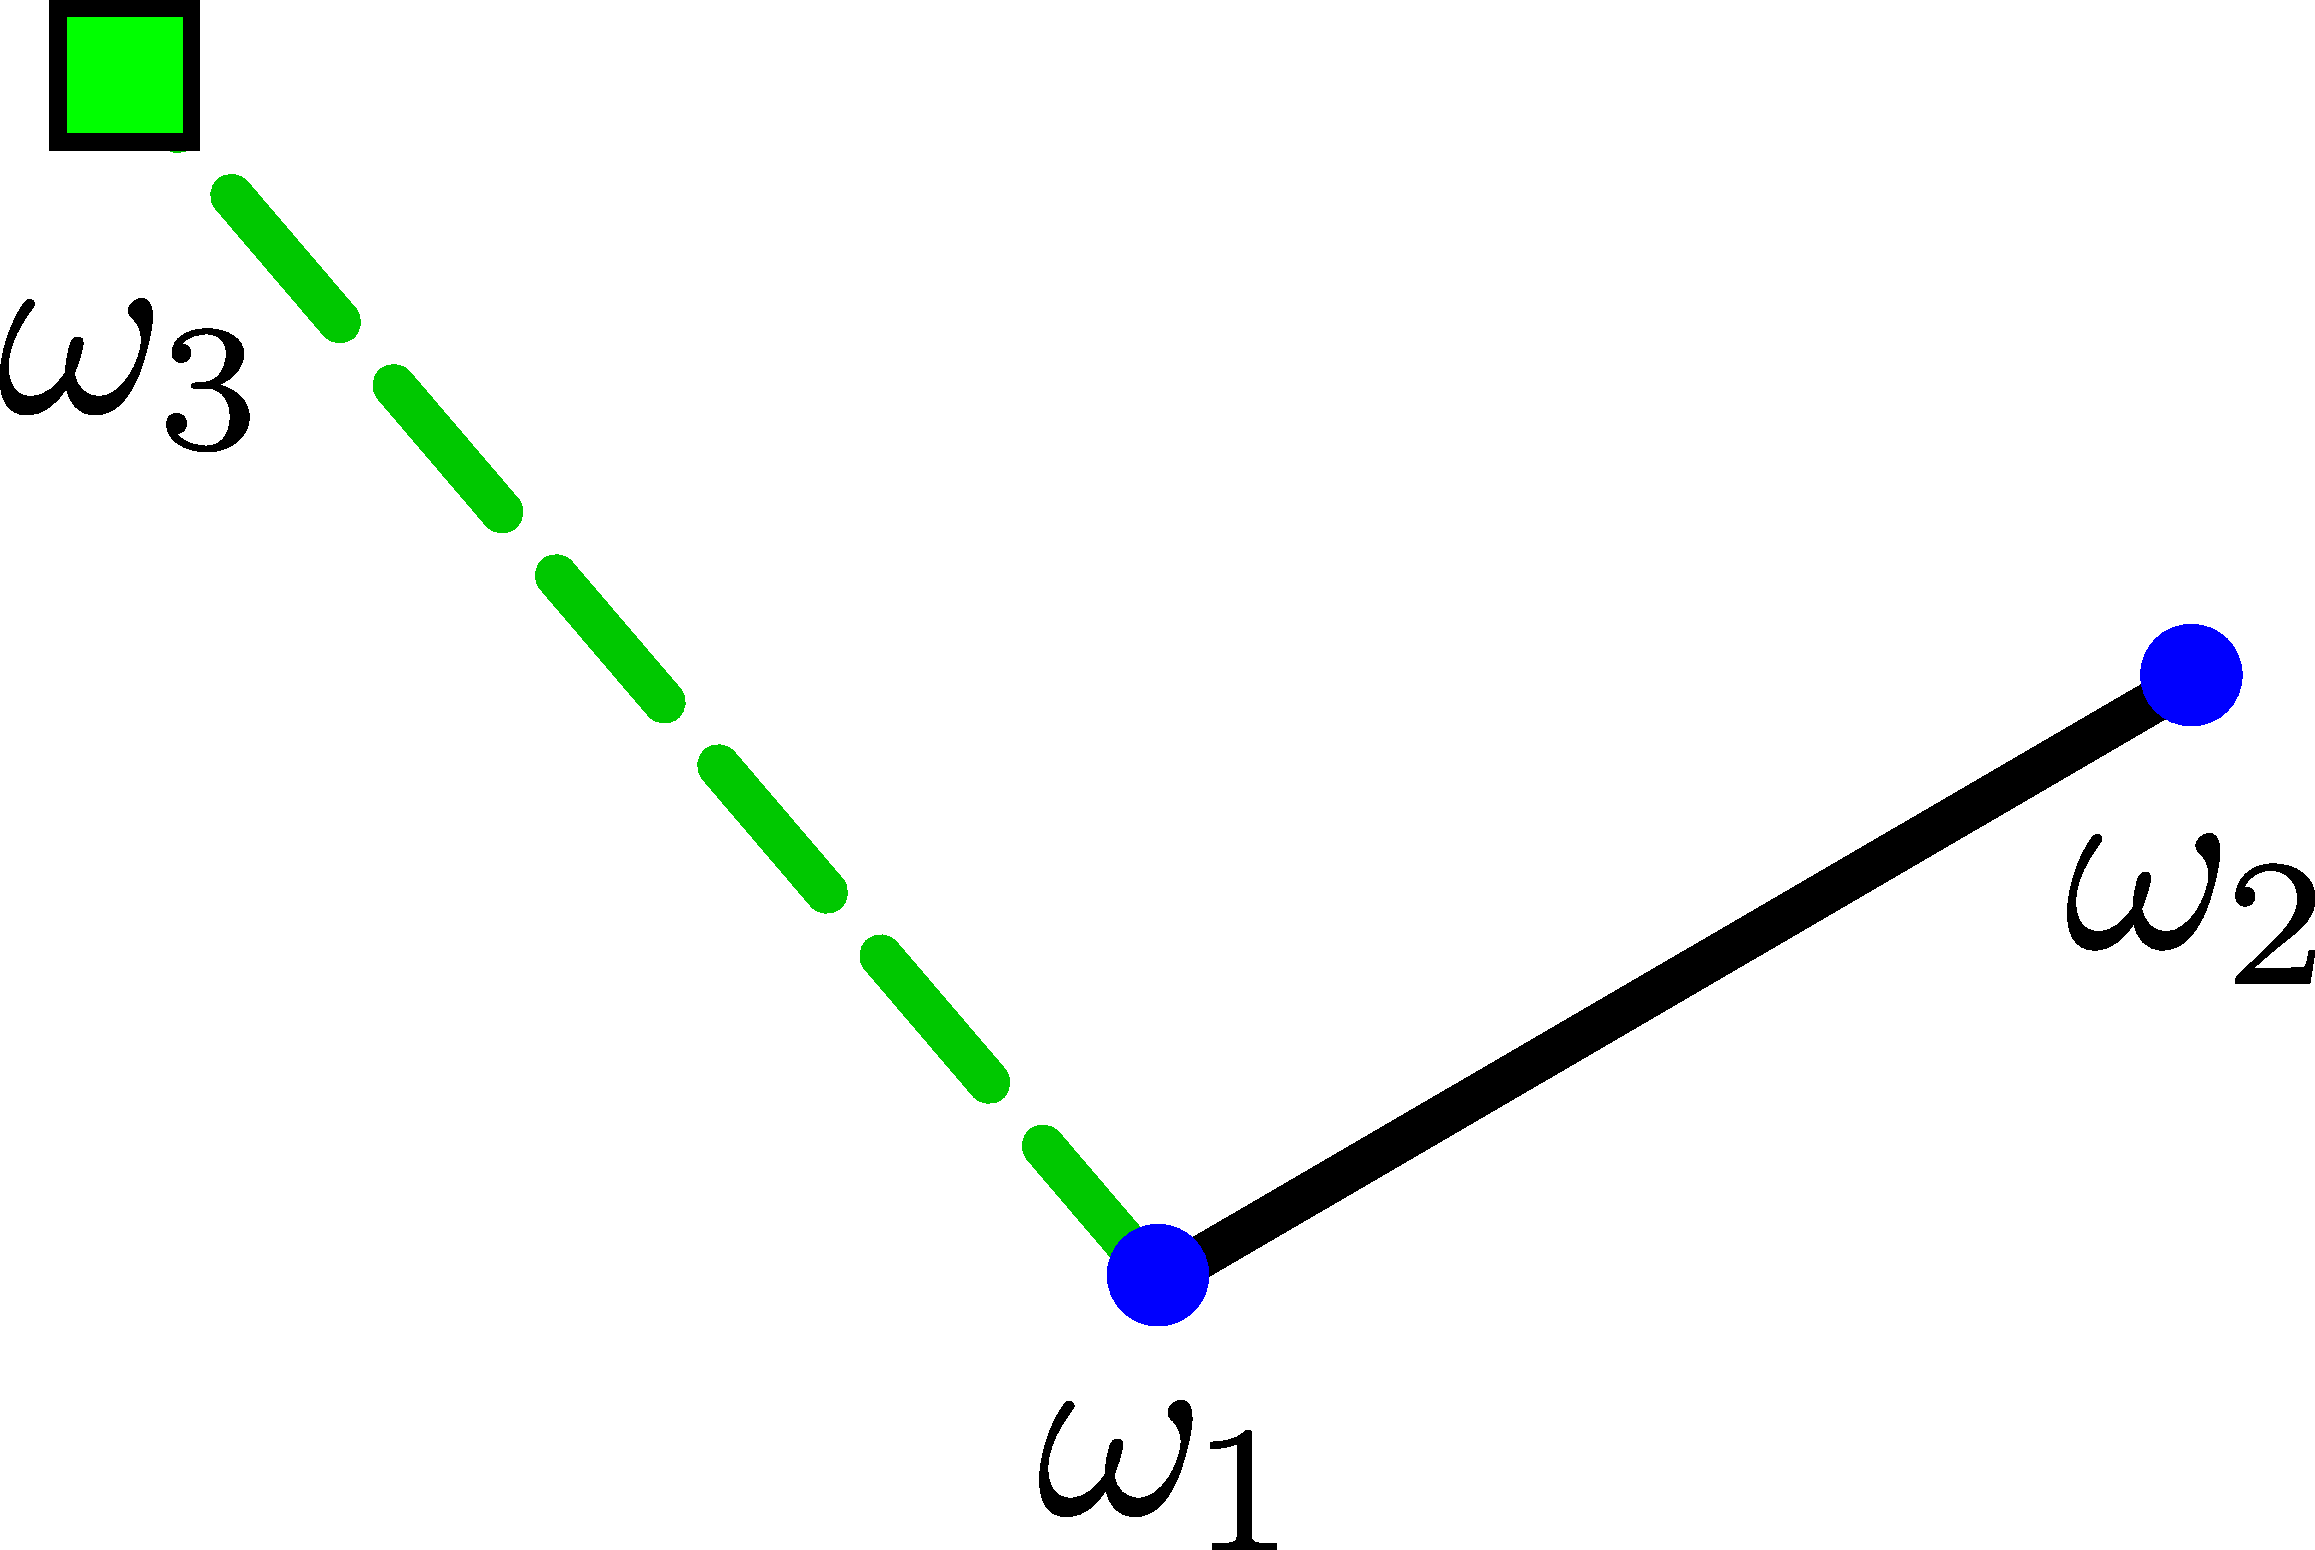
\includegraphics[scale=0.07]{Figures/LEI.pdf}}
      \label{fig:injLEI}
  \label{injLEI}
  \subfloat[Internal Injection]{
      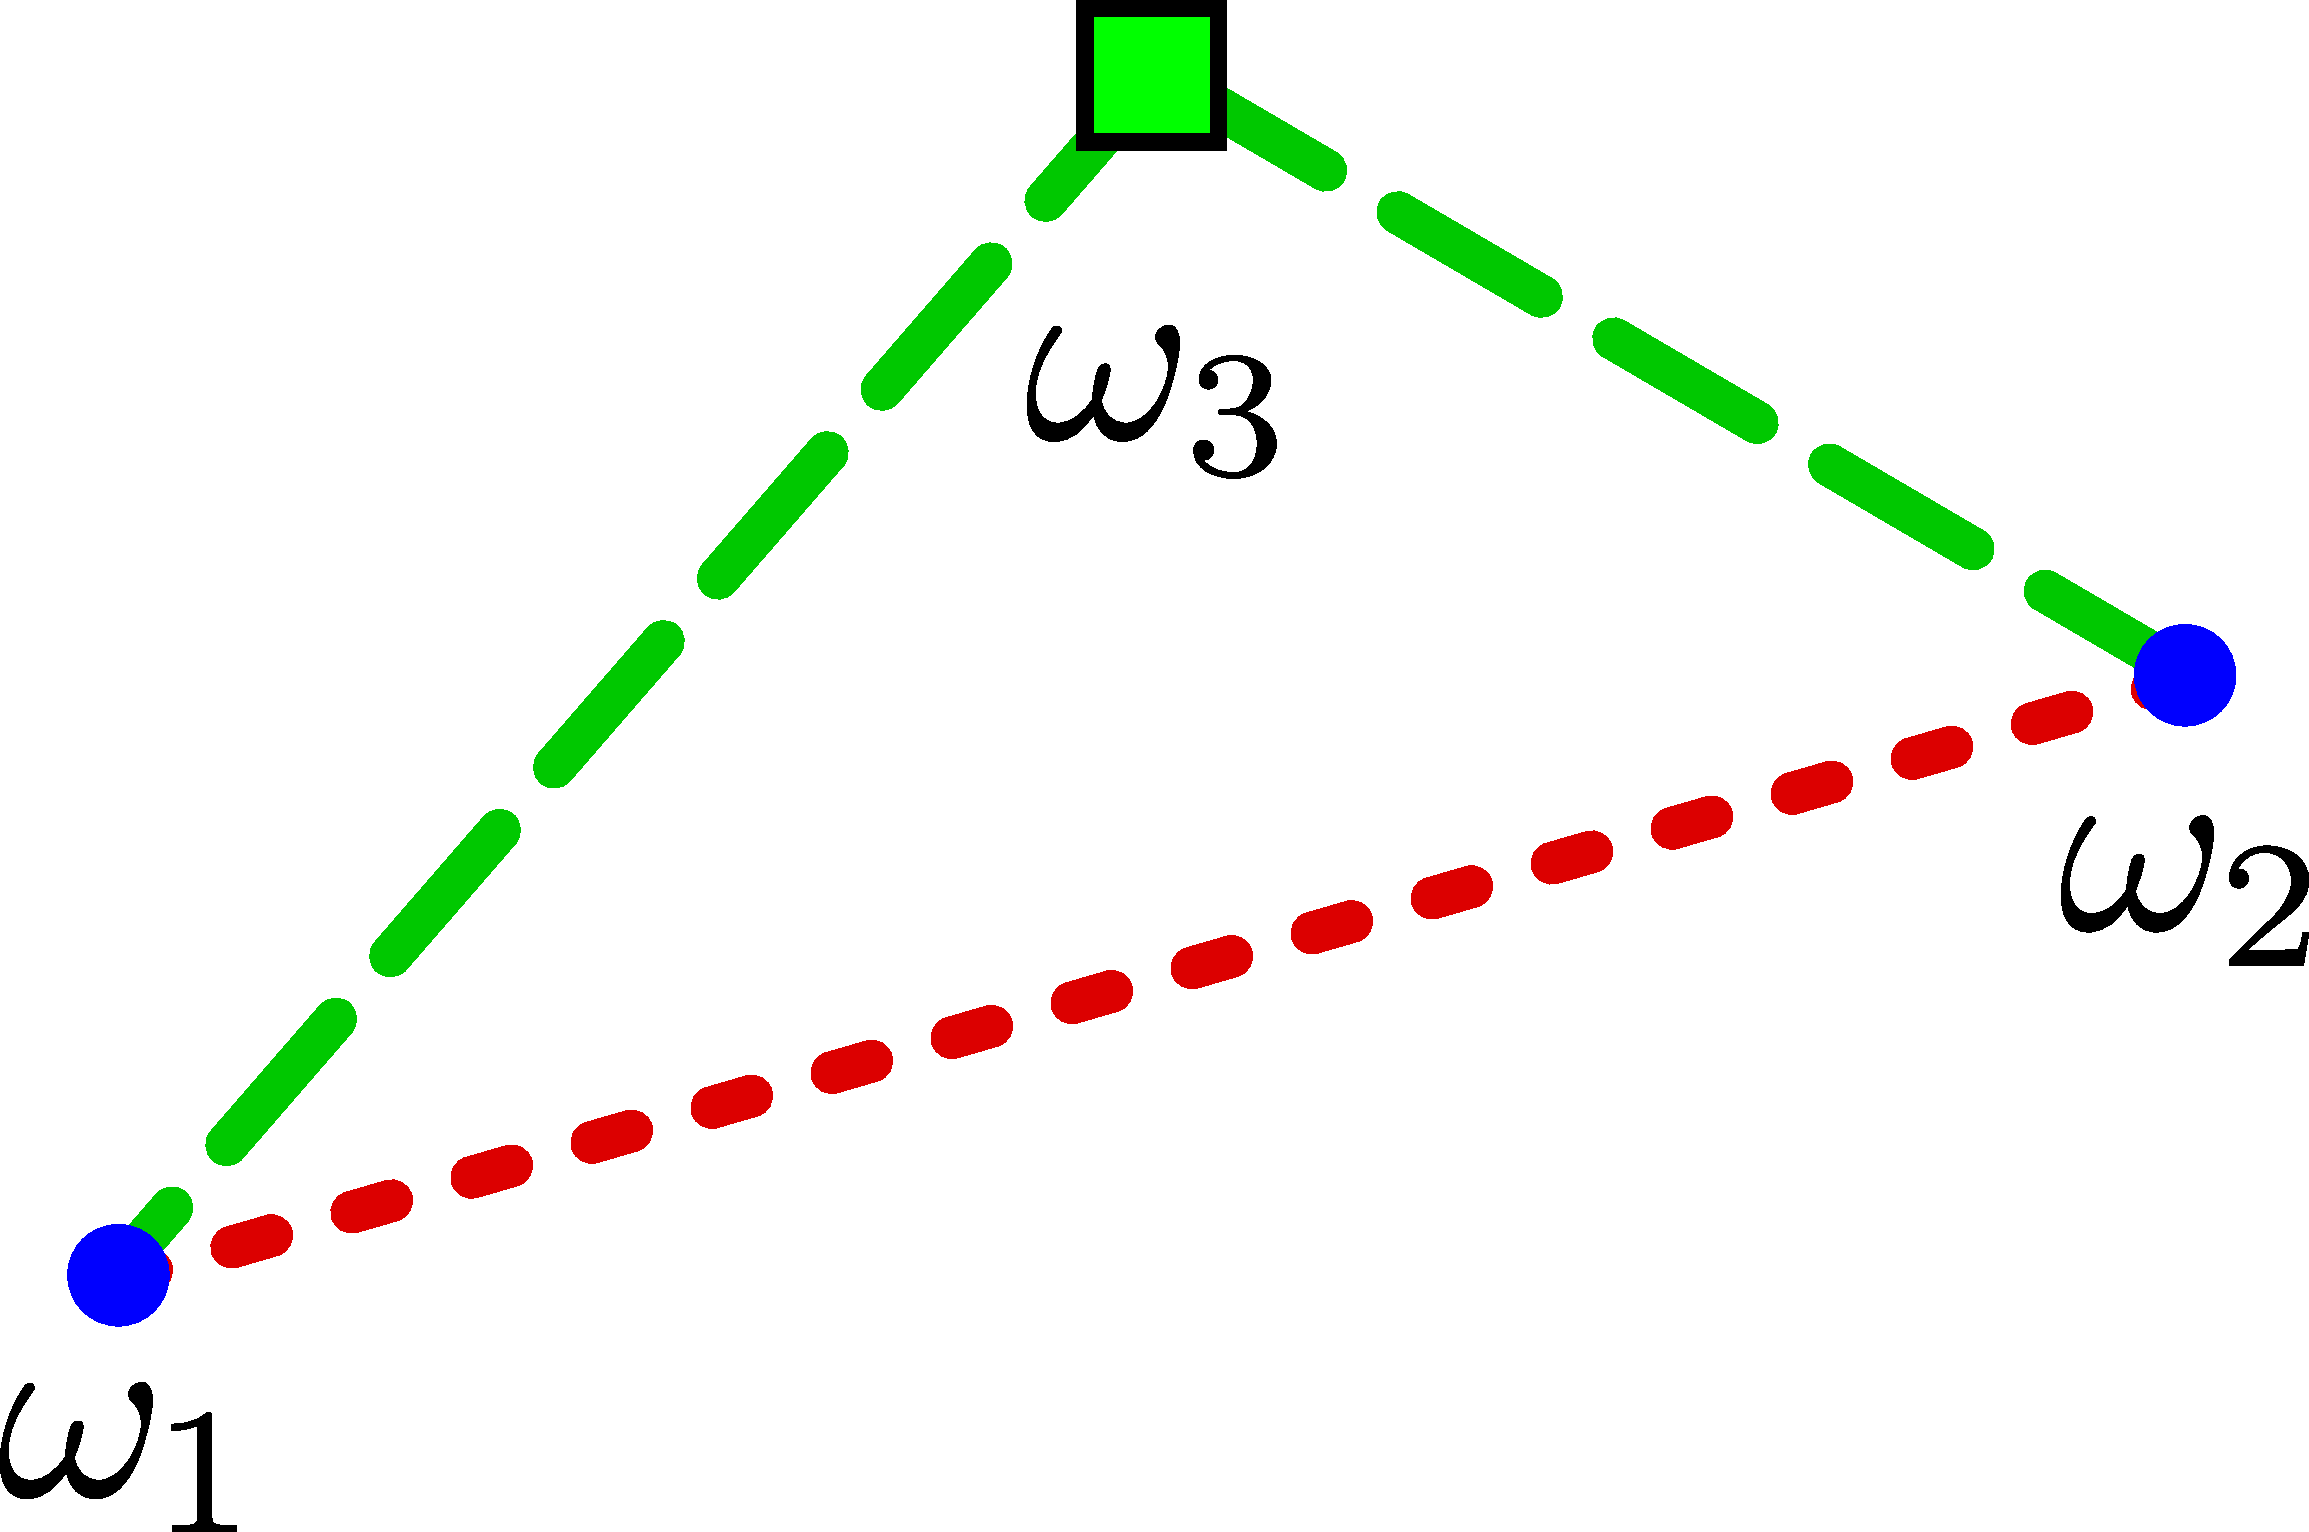
\includegraphics[scale=0.07]{Figures/II.pdf}}
      \label{fig:injII}
  \label{injII}
  \subfloat[Final Injection]{
      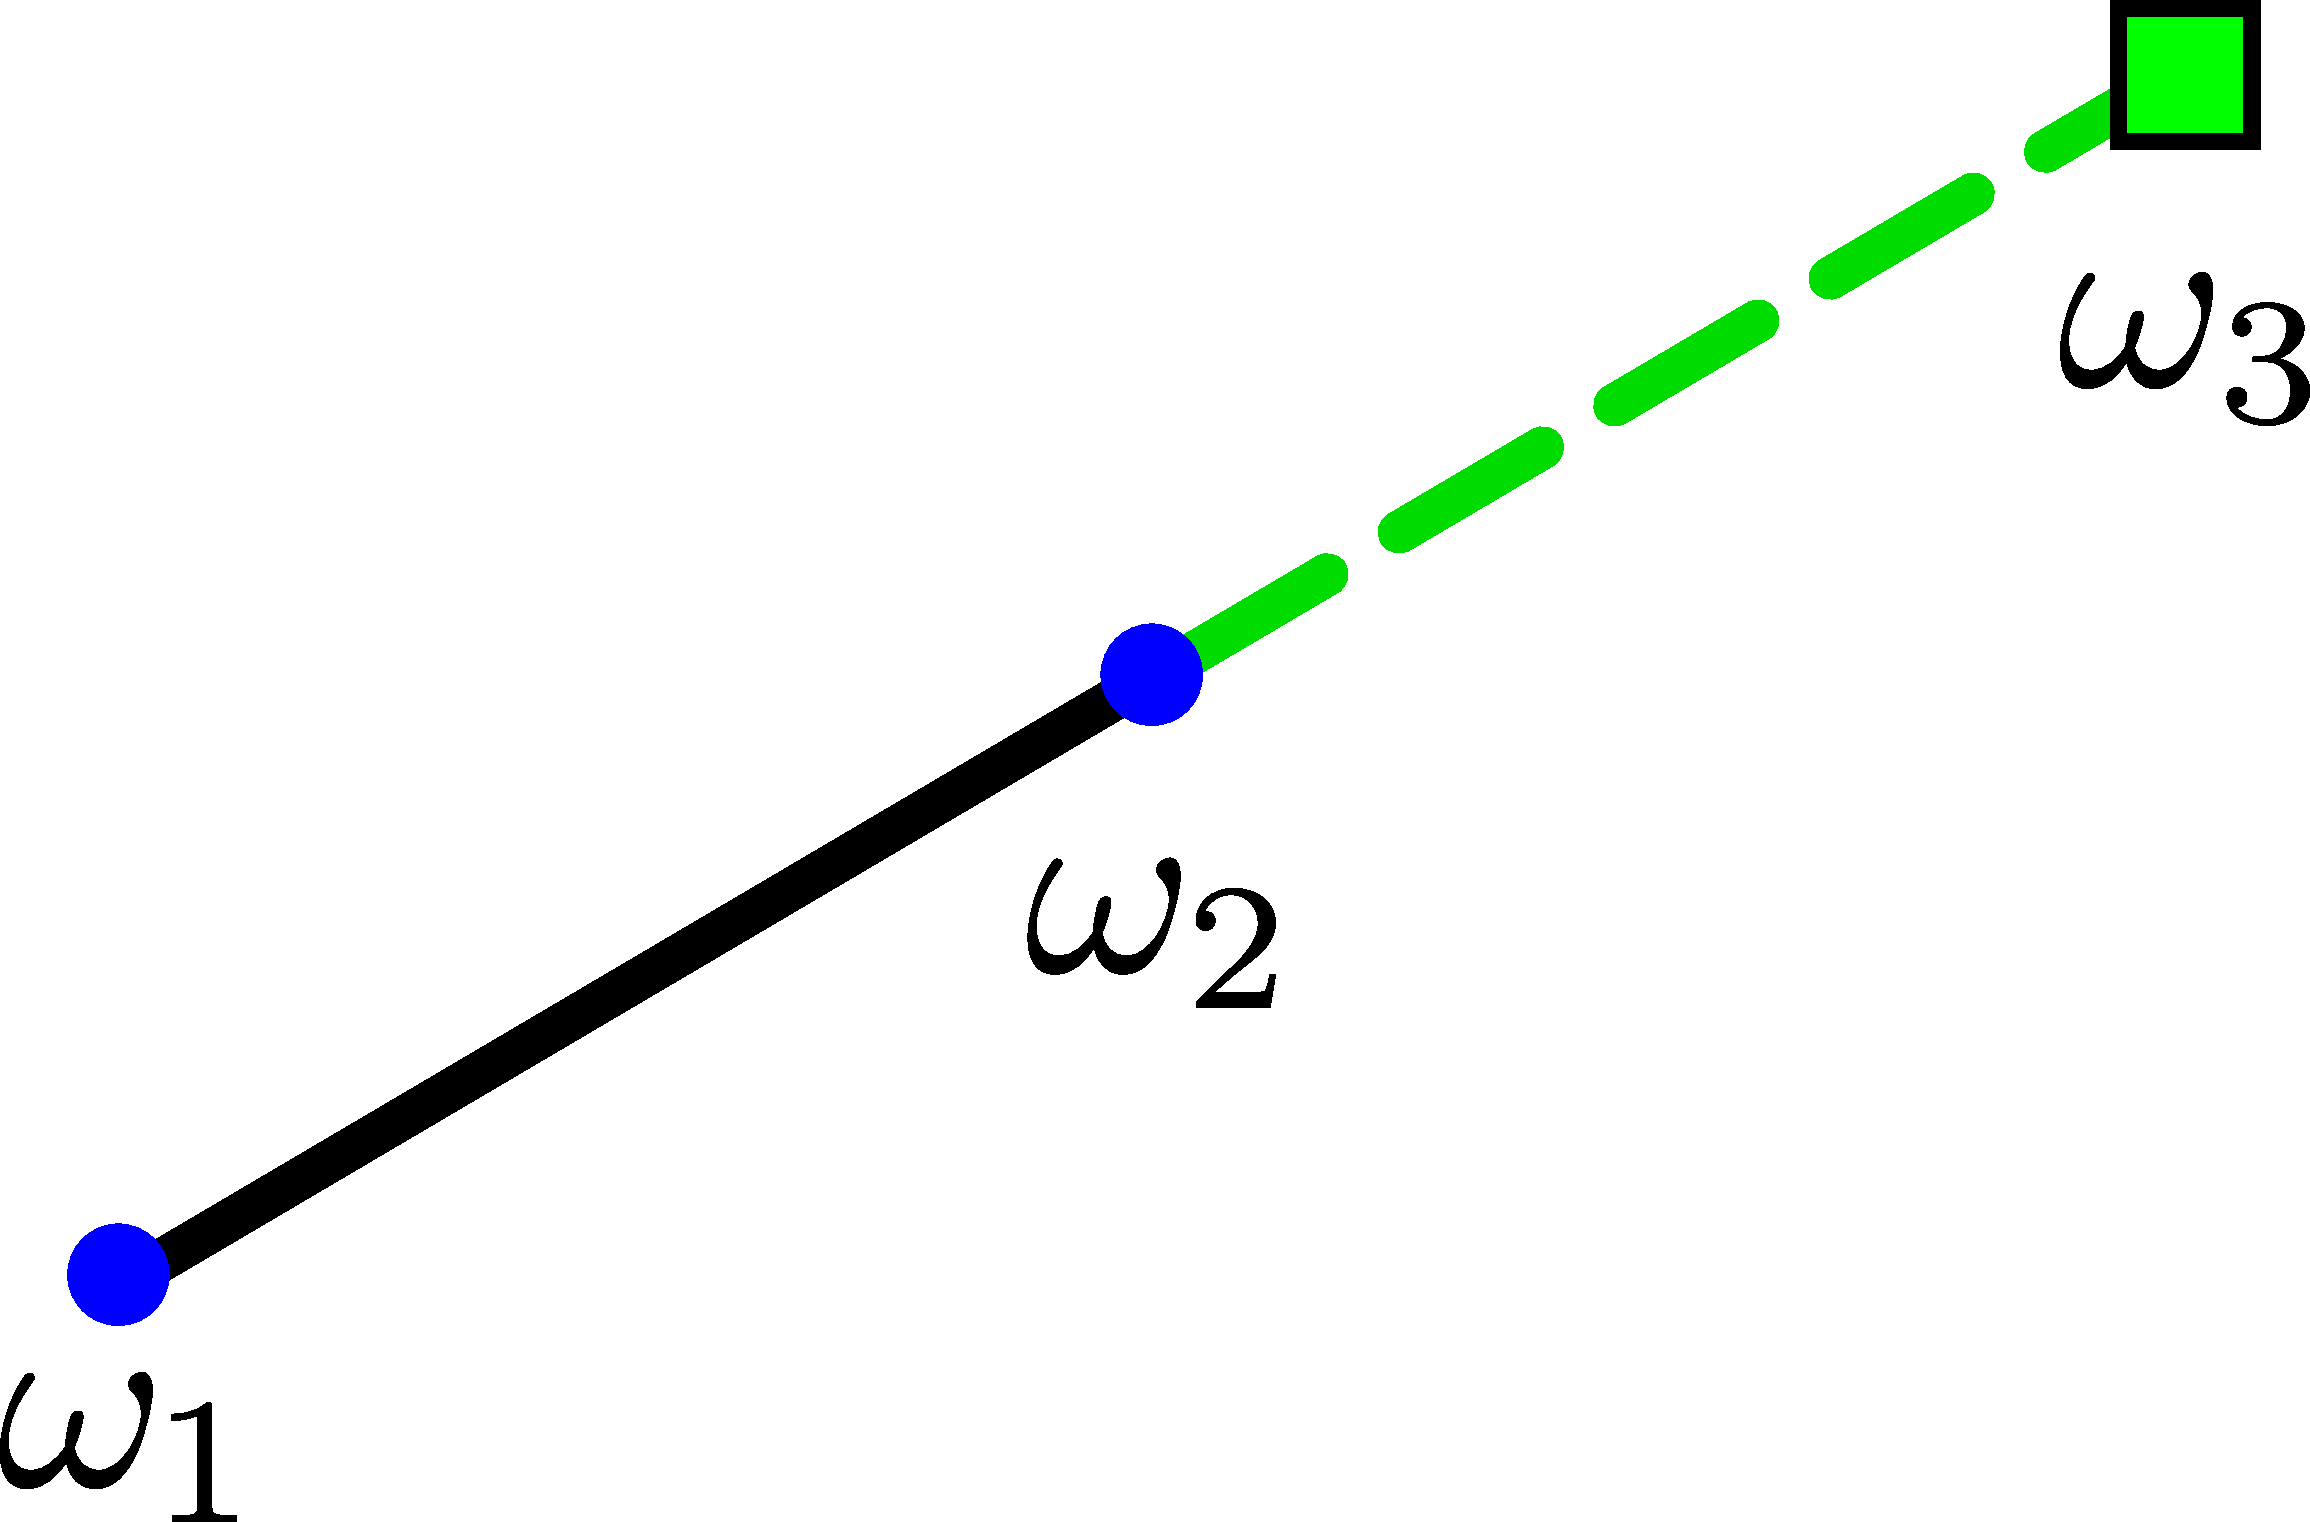
\includegraphics[scale=0.07]{Figures/FEI.pdf}}
      \label{fig:injFEI}
  \label{injFEI}
%\caption{A two-speed sequence, $\omega_1, \omega_2$, shown in blue dots, receives a(n) (a) leading injection, (b) internal injection, and (c) final injection by $\omega_3$ (green square). Dashed green lines, dotted red lines, and solid black lines represent the added minimum inter-arrival times, removed minimum inter-arrival times, and unchanged minimum inter-arrival times, respectively. Green squares represent the injected speed $\omega_3$.}
\caption{A two-speed sequence, $\omega_1, \omega_2$, shown as dots, receives the (a) leading, (b) internal, and (c) final, injection of $\omega_3$ shown as a square. Dashed, dotted, and solid lines represent the added, removed, and unchanged minimum inter-arrival times, respectively.}
\label{fig:injections}
\end{figure}

To compare the demand produced by two different sequences (with the same elements, but in different order), we will look at the time of the absolute deadline of the last job in the sequence under the assumptions that jobs of the sequence arrive according to their minimum interarrival time (i.e., $\widetilde{T}$) and the first job is released at time instant zero.   Let $d(S)$ be the last absolute deadline for sequence $S = (\omega_1, \ldots, \omega_n)$:
\begin{equation} \label{eq:speedSequenceTimeImplicitDeadline}
d(S) = \sum\limits_{i=1}^{n-1} \widetilde{T}(\omega_i,\omega_{i+1}) + \Tilde{d}(\omega_n).
\end{equation}

We can quantify how the $d(S)$ function changes as we inject elements of non-decreasing speed.  Let $\Delta(S, k, k+1)$ represent the amount that the $d$ function increases when injecting the $(k+1)^{th}$ smallest element ($s_{k+1}$) into $S(k)$.  That is,
\begin{equation} \label{eq:seq-delta}
\Delta(S, k, k+1) = d(S(k+1)) - d(S(k)).
\end{equation}

We can compute the above difference based on the type of injection that adding the $(k+1)^{th}$ smallest element to $S(k)$ results in:
\begin{equation} \label{eq:seq-delta-types}
\Delta(S, k, k+1) = \left\{
    \begin{array}{ll}
         \Delta_L (S, k, k+1)&{\rm if~leading},  \\
         \Delta_F (S, k, k+1)&{\rm if~final},\\
        \Delta_I (S, k, k+1)&{\rm if~internal},
    \end{array}
\right.
\end{equation}

\noindent where $\Delta_L (S, k, k+1) = \widetilde{T}(s_{k+1},\omega^{(k)}_1)$ since we are adding one segment to the front of $S(k)$ in the leading injection;   $\Delta_F (S, k, k+1) = \widetilde{T}(\omega^{(k)}_k, s_{k+1}) + \Tilde{d}(s_{k+1}) - \Tilde{d}(\omega^{(k)}_k)$ since we are adding one segment to the end of $S(k)$ and adjusting the deadline of the last job for the new speed $s_{k+1}$ for a final injection; and $\Delta_I (S, k, k+1) = \widetilde{T}(\omega^{(k)}_{j-1}, s_{k+1}) + \widetilde{T}(s_{k+1}, \omega^{(k)}_{j}) - \widetilde{T}(\omega^{(k)}_{j-1}, \omega^{(k)}_{j})$ if we inject $s_{k+1}$ into the $j^{th}$ position of $S(k)$, $j\in\mathbb{N}_2^{k}$.

We are now prepared to compare the amount of time added to the absolute deadline of the last job of the sequence, considering $k$-subsequences $S$ and $S_A$ and injecting the $(k+1)^{th}$ smallest element ($s_{k+1}$) into both of these sequences for each of the three types of injections.

\begin{property}[Leading Injection Suboptimality]\label{prop:ascending-dominates-L}
For any valid, finite sequence $S = (\omega_1, \ldots, \omega_n)$, for all $k = 1, \ldots, n-1$:
\begin{equation}\label{eqn:compare-delta-L}
    \Delta_L(S,k,k+1) \geq \Delta_F(S_A, k, k+1).
\end{equation}
\end{property}
\begin{proof}
In this property, we have a leading injection into $S(k)$.  However, observe that $\widetilde{d}(s_{k+1}) \leq \widetilde{d}({s_k})$ by Property~\ref{prop:deadline-derivative} and since $s_{k+1}$ is larger than any element of $S(k)$.  Furthermore, $\widetilde{T}(\omega^{(k)}_k, s_{k+1}) \geq \widetilde{T}(s_k, s_{k+1})$ since, by Property~\ref{prop:neg-deriv-min-interarrival}, $\widetilde{T}$ is a decreasing function in its parameters and $s_k$ is at least as large as any item in $S(k)$.  Also, by Property~\ref{T-reversal}, $\widetilde{T}(\omega^{(k)}_k, s_{k+1})$ equals $\widetilde{T}(s_{k+1}, \omega^{(k)}_k)$.  By the above observations, we get:
\begin{equation}\label{eq:FEIdominatesLEI}
\begin{array}{ll}                  
    & \widetilde{T}(s_{k+1}, \omega^{(k)}_k) +\Tilde{d}(s_k) \geq \widetilde{T}(s_k, s_{k+1})+\Tilde{d}(s_{k+1})\nonumber\\
    \Leftrightarrow & \widetilde{T}(s_{k+1}, \omega^{(k)}_k) \geq \widetilde{T}(s_k, s_{k+1})+\Tilde{d}(s_{k+1})- \Tilde{d}(s_k)\nonumber
\end{array}
\end{equation}

The LHS and RHS of the last inequality matches  Equation~\ref{eqn:compare-delta-L} and the lemma is proved.
\end{proof}



\begin{property}[Internal Injection Suboptimality]\label{prop:ascending-dominates-I}
For any valid, finite sequence $S = (\omega_1, \ldots, \omega_n)$, for all $k = 1, \ldots, n-1$:
\begin{equation}\label{eqn:compare-delta-I}
    \Delta_I(S,k,k+1) \geq \Delta_F(S_A, k, k+1).
\end{equation}
\end{property}
\begin{proof}
Observe that by Properties~\ref{T-reversal} and~\ref{prop:deadline-derivative}, $\widetilde{T}(f,\omega + \epsilon) \geq \tilde{d}(\omega + \epsilon)$ for all $f, \omega$ and $\epsilon > 0$.  Also, $\widetilde{T}(s_k +\epsilon, \omega) = \widetilde{T}(\omega, s_k+\epsilon)$ for all $\omega$ and $\epsilon >0$ by Property~\ref{T-reversal}. These properties imply that:
\begin{equation}\label{eqn:change-sk}
\begin{array}{ll}
     & 
     \begin{array}{ll}
        \lefteqn{\widetilde{T}(s_{k-1},s_k) + \widetilde{T}(s_k, s_k) + \tilde{d}(s_k)}& \\
            &= \widetilde{T}(s_{k-1},s_k) + \widetilde{T}(s_k,s_k) + \tilde{d}(s_k)
      \end{array}\\
     \Rightarrow & 
     \begin{array}{ll}
        \lefteqn{\widetilde{T}(s_{k-1},s_k +\epsilon) + \widetilde{T}(s_k+\epsilon, s_k) + \tilde{d}(s_k)}& \\
        &\geq \widetilde{T}(s_{k-1},s_k) + \widetilde{T}(s_k, s_k + \epsilon) + \tilde{d}(s_k+\epsilon) 
    \end{array}\\
\end{array}
\end{equation}

\noindent Setting $\epsilon = s_{k+1} - s_k$ and substituting into the above inequality of Equation~\ref{eqn:change-sk}, we get the following:
\begin{equation}\label{eqn:change-sk2}
\begin{array}{ll}
     &\begin{array}{ll}
        \lefteqn{\widetilde{T}(s_{k-1},s_{k+1}) + \widetilde{T}(s_{k+1}, s_k) + \tilde{d}(s_k)}& \\
        &\geq \widetilde{T}(s_{k-1},s_k) + \widetilde{T}(s_k, s_{k+1}) + \tilde{d}(s_{k+1}) 
    \end{array}\\
    \Rightarrow&
    \begin{array}{ll}
        \lefteqn{\widetilde{T}(s_{k-1},s_{k+1}) + \widetilde{T}(s_{k+1}, s_k) - \widetilde{T}(s_{k-1},s_k)}& \\
        &\geq \widetilde{T}(s_k, s_{k+1}) + \tilde{d}(s_{k+1}) - \tilde{d}(s_k)
    \end{array}\\
    \Rightarrow&
    \begin{array}{ll}
        \lefteqn{\widetilde{T}(\omega^{(k)}_{j-1}, s_{k+1}) + \widetilde{T}(s_{k+1},\omega^{(k)}_{j}) - \widetilde{T}(\omega^{(k)}_{j-1},\omega^{(k)}_{j})} &\\
        &\geq \widetilde{T}(s_k, s_{k+1}) + \tilde{d}(s_{k+1}) - \tilde{d}(s_k) \\
    \end{array}\\
\end{array}
\end{equation}
% \sandeep{Why are we only changing $s_k$ to $\omega^{(k)}_{j}$ on the left hand side of the last inequality and not the right side?}
\noindent The last inequality (which implies Equation~\ref{eqn:compare-delta-I} of the property) above follows from observing that according to Property~\ref{prop:neg-deriv-min-interarrival}, the following is true for all $\omega$ and $\omega'$:
\begin{equation}
\begin{array}{ll}
        &\frac{\partial \widetilde{T}(\omega,s_{k+1})}{\partial \omega}
            \leq \frac{\partial \widetilde{T}(\omega,\omega')}{\partial \omega} \nonumber\\
        \Leftrightarrow&
        \frac{\partial \widetilde{T}(\omega,s_{k+1})}{\partial \omega} + \frac{\partial \widetilde{T}(s_{k+1},\omega')}{\partial \omega} - \frac{\partial \widetilde{T}(\omega,\omega')}{\partial \omega} \leq 0 \nonumber  
\end{array}
\end{equation}
\noindent  Thus, the LHS of the second inequality of Equation~\ref{eqn:change-sk2} will not decrease if we substitute $\omega^{(k)}_{j-1}$ for $s_{k-1}$ in the LHS.  For symmetric reasons, we can also substitute $\omega^{(k)}_{j}$ for $s_k$.
\end{proof}

%\fishern{Making a pass from this point -- 1:10am 6/1}

In this next property, we show that any sequence may decrease the time of its last deadline by moving the highest speed job to the end (if it is valid).  The proof of this property is in the appendix.

\begin{property}[Highest-Speed Relative-Deadline Dominance]\label{prop:high-speed-transfer}
For any valid, finite sequence $S = (\omega_1, \ldots, \omega_n)$, if $\omega_\ell$ ($\ell \in \mathbb{N}_1^n-1$) is the highest speed $s_n$ and not the last speed of sequence $S$ and $s_n \leq \Omega_1(\omega_n,\alpha_{\max})$ then new sequence $S'$ with the highest element moved to the last element (i.e., $S' = (\omega_1, \ldots, \omega_{\ell-1}, \omega_{\ell+1}, \ldots, \omega_n, s_n)$) is valid and has the following property: 
\begin{equation}\label{eqn:high-speed-transfer}
    d(S) \geq d(S').
\end{equation}
\end{property}

We are now ready to state the main lemma of this subsection.  That is, for any dominant speed sequence, we can find another dominant speed sequence with equivalent demand that is in ascending order.

\begin{lemma}[Dominant Non-Decreasing Speed Sequences]\label{lemma:non-decreasing}
Given a valid, dominant speed sequence $S = (\omega_1, \omega_2, \ldots, \omega_n)$ over interval $[t_a, t_b]$, the sequence $S_A$ is valid and has equivalent demand.
\end{lemma}
\begin{proof}
The proof is by induction on $k$.  For each $k \in \mathbb{N}_1^n$, we show that for any $k$-subsequence $S'(k)$ containing the same elements of $S(k)$ such that $d(S(k)) \geq d(S'(k))$, the following is true:
\begin{equation}\label{eqn:non-decr-IH}
    d(S(k)) \geq d(S'(k)) \geq d(S_A(k)).
\end{equation}
\noindent This implies the lemma, since if the deadline of the last job of $S$ is before $t_b$, then the last job of $S_A$ must also be before $t_b$; therefore, the demand over the interval does not decrease when reordering $S$ to non-decreasing order.
 
\noindent \emph{Base Case}: Consider when $k=1$, clearly $S(1)=S_A(1) = (s_1)$.  Thus, Equation~\ref{eqn:non-decr-IH} is vacuously true.

\noindent \emph{Induction Hypothesis}:  Assume that Equation~\ref{eqn:non-decr-IH} holds up to some $k < n$ for all $S'(k)$ containing the same elements of $S(k)$ such that $d(S(k)) \geq d(S'(k))$.

\noindent \emph{Inductive Step}:  We need to show that Equation~\ref{eqn:non-decr-IH} is true for $k+1$.  Let $S'(k)$ be any $k$-subsequence.  We now consider injecting $s_{k+1}$ into $S'(k)$ and $S_A(k)$.  (Note that $S_A$ and $S'_A$ are identical subsequences).  There are three cases depending on the type of injection into $S'(k)$.
\begin{case}[Leading Injection]
  By Property~\ref{prop:ascending-dominates-L}, $\Delta_L(S',k,k+1) \geq \Delta_F(S_A,k,k+1)$.  Therefore, by the Induction Hypothesis, $d(S'(k+1)) = d(S'(k))+ \Delta_L(S',k,k+1)\geq d(S_A(k)) + \Delta_F(S_A,k, k+1) = d(S_A(k+1))$.  
\end{case}
\begin{case}[Internal Injection]
  By Property~\ref{prop:ascending-dominates-I}, $\Delta_I(S',k,k+1) \geq \Delta_F(S_A,k,k+1)$.  Therefore, by the Induction Hypothesis, $d(S'(k+1)) = d(S'(k))+ \Delta_I(S',k,k+1)\geq d(S_A(k)) + \Delta_F(S_A,k, k+1) = d(S_A(k+1))$.  
\end{case}
\begin{case}[Final Injection]
  By Property~\ref{prop:high-speed-transfer}, there exist a valid sequence $S''(k)$ obtained from $S'(k)$ by moving the highest term ($s_k$) to the end of $S''(k)$ where $d(S'(k))\geq d(S''(k))$.   (If $S'(k)$ already had $s_k$ as its last term, then $S''(k) = S'(k)$).  By Induction Hypothesis, $d(S''(k)) \geq d(S_A(k))$.
  Since the last term on $S'(k)$ and $S_A$ is identical, $\Delta_F(S',k, k+1)$ equals $\Delta_F(S_A,k,k+1)$.  Observe that $\Delta_F(S',k, k+1) \geq \Delta_F(S'', k, k+1)$ since the last element in $S''$ is $s_k$ and Property~\ref{prop:deadline-derivative} implies $S''$ will have less time added to its deadline.  Therefore, we have $d(S'(k))+\Delta_F(S',k,k+1) \geq d(S''(k)) + \Delta_F(S'',k,k+1) \geq d(S_A(k)) + \Delta_F(S_A,k,k+1)$. Hence, $d(S'(k+1))\geq d(S_A(k+1))$.
\end{case}
In all the cases, we show that for all $S'$ such that $d(S(k+1)) \geq d(S'(k)) \Rightarrow d(S'(k)) \geq d(S_A(k))$ which proves the lemma.
\end{proof}






%%%%%%%%%%%%%%%%BEGIN COMMENT%%%%%%%%%%%%%%%%%%%%%
\begin{comment}
\paragraph{Speed Sets and Sequences}

The following model is established to describe speed sequences:
\begin{enumerate}
\item $\mathcal{S}$ is a \textit{Speed Set}, an ordered, finite set of speeds where $\mathcal{S}=(\omega_1, \omega_2, \omega_3,...,\omega_n) \quad | \quad \omega_i \leq \omega_j \quad \forall i<j$. 
\item $\mathcal{S}(k)$ is a \textit{Speed Subset}, an unordered, finite subset of $\mathcal{S}$ containing the $k$ lowest speeds in $\mathcal{S}$. More formally, $\mathcal{S}(k) \subseteq S \quad | \quad S(k) = \{s_1, s_2, ... , s_k\} : k \leq n$.
\item $Q(\mathcal{S}(k))$ is a \textit{Speed Sequence}, an ordered permutation of $\mathcal{S}$ where $Q(\mathcal{S}(k))=(q_1, q_2, q_3, ... , q_k)$ %\quad | \quad \forall i \in \mathbb{Z} \quad | \quad 0 < i < n$
\item $Q_{A}(\mathcal{S}(k))$ is an \textit{Ascending Speed Sequence}, an ordered permutation of $\mathcal{S}$ where $Q_{A}(\mathcal{S}(k))=(q_1, q_2, q_3, ... , q_k) \: | \: q_i = s_i \: \forall i \in \mathbb{N}_1 : 1 \leq i \leq k$
\item $\mathcal{Q}(S)$ is a \textit{Sequence Space}, a set of all ordered permutations of $\mathcal{S}$.
\item $\mathcal{Q}_{feasible}(\mathcal{S}(k))$ is a \textit{Feasible Sequence Space}, the set of all $Q(\mathcal{S}(k))$ where \\ $q_{i+1} \leq \sqrt{q_i^{2} + 2\alpha_{\max}} \quad \forall i \in \mathbb{Z} \: | \: 1 \leq i \leq n-1 \:$.
\end{enumerate}

\subsubsection{Speed Injections}
equations describe speed injections, sequence transformations for manipulating speed sequences by adding a speed $\omega_{k+1}$ to a $Q(\mathcal{S}(k))$.
\subparagraph{Leading External Injection}
A Leading External Injection is a transformation defined as:
\begin{equation}
\textbf{T}_{LEI}(Q(\mathcal{S}(k)),\omega_{k+1}) = Q'(\mathcal{S}(k+1)) \: | \: q'_1 = \omega_{k+1}
\end{equation}
%where $Q'(\mathcal{S}(k+1))$ has $\omega_{k+1}$ as the first speed.
which causes an increase in sequence time:
\begin{equation}\label{eq:injLeading}
\Delta t_{LEI}(Q(\mathcal{S}(k)),\omega_{k+1}) = m(\omega_{k+1},q_1)
\end{equation}
Note that Equation \ref{eq:injLeading} is minimized when $q_1 = \omega_k$.
\subparagraph{Internal Injection}
An Internal Injection is a transformation defined as:
\begin{equation}
\textbf{T}_{II}(Q(\mathcal{S}(k)),q_x,\omega_{k+1}) = Q'(\mathcal{S}(k+1)) \: | \: q'_{x+1} = \omega_{k+1}
\end{equation}
where $1 \leq x < k-1$ with the increase in sequence time:
\begin{alignat}{3} \label{eq:injInternal}
&\Delta t_{II}(Q(\mathcal{S}(k)),q_x,\omega_{k+1}) =& \nonumber \\
&m(q_x,\omega_{k+1}) + m(\omega_{k+1}, q_{x+1}) - m(q_x,q_{x+1})&
\end{alignat}
Note Equation \ref{eq:injInternal} is minimized when $q_x = \omega_k, q_{x+1} = \omega_{k-1}$.
\subparagraph{Final External Injection}
A Final External Injection is a transformation which inserts a speed into a sequence defined as:
\begin{equation}
\textbf{T}_{FEI}(Q(\mathcal{S}(k)),\omega_{k+1}) = Q'(\mathcal{S}(k+1)) \: | \: q'_k = \omega_{k+1}
\end{equation}
For final external injections, the increase in time is defined as:
\begin{alignat}{3}\label{eq:injFinal}
&\Delta t_{FEI}(Q(\mathcal{S}(k)),\omega_{k+1}) = \nonumber \\ &m(q_k,\omega_{k+1}) + E(\omega_{k+1}) - E(q_k)
\end{alignat}
Note that Final External Injection of $\omega_{k+1}$ into $Q_{A}(S(k))$ will maintain the ascending property of the sequence permutation.


\begin{lemma}[Dominant Non-Decreasing Speed Sequences]\label{lemma:non-decreasing}
Given a speed set, $\mathcal{S}$, of size $n$, the ascending speed sequence, $Q_{A}(S(k))$ in which speeds are traversed in increasing order gives the fastest speed sequence time. Formally, $\Delta_t(Q_{A}(S(k))) \leq \Delta_t(Q(S(k)) \: \forall k \in \mathbb{N}_1 : 1 \leq k \leq n, \; S(k), \; Q(S(k)) \in \mathcal{Q}_{feasible}(S(k))$.
\end{lemma}
\begin{proof}
\subparagraph{Base Case - $\Delta_t(Q(\mathcal{S}(1))) \leq \Delta_t(Q_{A}(\mathcal{S}(1)))$}
By Equations \ref{eqn:deadline-derivative} and \ref{eq:speedSequenceTimeImplicitDeadline}, an initial $Q_{A}(\mathcal{S}(1))$ is equivalent to any $Q(\mathcal{S}(1)) \in \mathcal{Q}_{feasible}(\mathcal{S}(1))$.
Since $\mathcal{S}(1)$ contains only one speed and has only one permutation, $Q(\mathcal{S}(1))$ is an ascending sequence such that $Q(\mathcal{S}(1)) = Q_{A}(\mathcal{S}(1))$.
Therefore, $\Delta_t(Q(\mathcal{S}(1))) \leq \Delta_t(Q_{A}(\mathcal{S}(1)))$, is true.
\subparagraph{Inductive Step - $Q(\mathcal{S}(k)) \leq Q_{A}(\mathcal{S}(k))$}
Given a speed set, $S$, and sequence permutation $Q(\mathcal{S}(k))$, the sequence permutation $Q(\mathcal{S}(k))$ can be constructed via a series of transformations: Leading External, Internal, or Final External speed injections. For example, $Q(\mathcal{S}(1))$ may be transformed into $Q(\mathcal{S}(2))$ via Equations \ref{eq:injLeading} or \ref{eq:injFinal}: $\textbf{T}_{LEI}(Q(\mathcal{S}(1)),\omega_{2})$ or $\textbf{T}_{FEI}(Q(\mathcal{S}(k)),\omega_{k+1})$. However, $Q(\mathcal{S}(2))$ contains too few elements yet for Equation \ref{eq:injInternal}, $\textbf{T}_{II}(Q(\mathcal{S}(1)),q_x,\omega_{2})$.

The following cases compare and establish dominant sequence transformations and sequences:
\begin{case}[Minimum Leading External Injection]
Ascending Final External Injection into $Q_{A}(\mathcal{S}(k))$ adds less time than ascending Leading External Injection to any $Q(\mathcal{S}(k))$.
\end{case}
Suppose $Q(\mathcal{S}(k))$ is ordered such that $q_1 = \omega_k$ in Equation \ref{eq:injLeading}. $\Delta t_{FEI}(Q_{A}(\mathcal{S}(k)),\omega_{k+1})$ will be minimized for all possible $q_1$ and compares as follows:
\begin{alignat}{4} \label{eq:FEIdominatesLEI}
&& E(\omega_k) & \geq E(\omega_{k+1}) &\quad& \nonumber \\
\Leftrightarrow && \widetilde{T}(\omega_{k+1},q_1) + E(\omega_k) & \geq \widetilde{T}(\omega_k,\omega_{k+1}) + E(\omega_{k+1}) &\quad& \nonumber \\
\Leftrightarrow && \widetilde{T}(\omega_{k+1},q_1) & \geq \widetilde{T}(\omega_k,\omega_{k+1}) + E(\omega_{k+1}) &\quad& \nonumber \\
\Leftrightarrow && \Delta t_{LEI}(Q(\mathcal{S}(k)),\omega_{k+1}) & \geq \Delta t_{FEI}(Q_{A}(\mathcal{S}(k)),\omega_{k+1}) && %\\
%&& & \qquad \qquad \qquad \text{By Eq. \ref{eq:injFinal}} \nonumber
\end{alignat}

\begin{case}[Minimum Internal Injection]\label{case:optimalInternalInjection}
Ascending final external injection adds less time to $Q_{A}(\mathcal{S}(k))$ than ascending internal external injection to any $Q(\mathcal{S}(k))$.
\end{case}
Suppose $Q(\mathcal{S}(k))$ is ordered such that $q_x = \omega_{k-1}, q_{x+1} = \omega_{k+1}$ in Equation \ref{eq:injInternal}. $\Delta t_{II}(Q(\mathcal{S}(k)),q_x,\omega_{k+1})$ will be minimized for all possible $q_x, q_{x+1}$ and compares as follows.
Let $a = \omega_{k-1}$, $b = c = \omega_k$, and $\delta = \omega_{k+1}-\omega_k$ and compare a partial increase $\delta$ in $b$ versus $c$ by the following equations:
\begin{alignat}{4}\label{eq:FEIdominatesII}
&& \widetilde{T}(a,b) + \widetilde{T}(b,c) + E(c) & = \widetilde{T}(a,b) + \widetilde{T}(b,c) + E(c) & \nonumber \\
\Leftrightarrow && \widetilde{T}(\omega_{k-1},\omega_k) + \widetilde{T}(\omega_k,\omega_k) + E(\omega_k) & = \widetilde{T}(\omega_{k-1},\omega_k) + \widetilde{T}(\omega_k,\omega_k) + E(\omega_k) & \nonumber \\
\Leftrightarrow && \widetilde{T}(\omega_{k-1},\omega_k+\delta) + \widetilde{T}(\omega_k+\delta,\omega_k) + E(\omega_k) & \geq \widetilde{T}(\omega_{k-1},\omega_k) + \widetilde{T}(\omega_k,\omega_k+\delta) + E(\omega_k+\delta) & \nonumber \\
\Leftrightarrow && \widetilde{T}(\omega_{k-1},\omega_{k+1}) + \widetilde{T}(\omega_{k+1},\omega_k) + E(\omega_k)& \geq  \widetilde{T}(\omega_{k-1},\omega_k) + \widetilde{T}(\omega_k,\omega_{k+1}) + E(\omega_{k+1}) & \nonumber \\
\Leftrightarrow && \widetilde{T}(q_x,\omega_{k+1}) + \widetilde{T}(\omega_{k+1},q_{x+1}) - \widetilde{T}(\omega_{k-1},\omega_k) & \geq  \widetilde{T}(\omega_k,\omega_{k+1}) + E(\omega_{k+1}) - E(\omega_k) & \nonumber \\
\Leftrightarrow && \Delta t_{II}(Q(\mathcal{S}(k)),q_x,\omega_{k+1}) & \geq \Delta t_{FEI}(Q_{A}(\mathcal{S}(k)),\omega_{k+1}) &\quad& \text{By Eq. \ref{eq:injFinal}}
\end{alignat}

\begin{case}[Highest Speed Transfers for $q_k \neq \omega_k$] Highest Speed Transfers are time-reducing transformations which apply to sequences where $q_k \in Q(\mathcal{S}(k)) \neq \omega_k$. If $\textbf{T}_{HST}(Q(\mathcal{S}(k))$ is infeasible, $\textbf{T}_{FEI}(Q(\mathcal{S}(k),\omega_{k+1})$ is also infeasible.
\end{case}
\begin{proof}
By Equation \ref{eq:HST}, Highest Speed Transfers transform $Q(\mathcal{S}(k))$ into $Q'(\mathcal{S}(k)) \:|\: q'_k = \omega_k$ and all transfers are time-reducing by Lemma \ref{lem:HST}. However, this transformation is feasible only when the highest speed $\omega_k$ is reachable from the final speed $q_k$ such that $\omega_k \leq \sqrt{q_k^2 + 2\alpha_{\max}}$. If $\textbf{T}_{HST}(Q(\mathcal{S}(k))$ is infeasible, $\omega_k > \sqrt{q_k^2 + 2\alpha_{\max}} \implies \omega_{k+1} > \sqrt{q_k^2 + 2\alpha_{\max}}$ since $\omega_k \leq \omega_{k+1}$ by the definition of $\mathcal{S}(k)$.
\end{proof}
\begin{case}[Equivalent Final External Injection] Ascending final external injection into $Q_{A}(\mathcal{S}(k))$ adds time equal to ascending internal external injection to any $Q(\mathcal{S}(k))$.
\end{case}
\begin{proof}
Suppose the final jobs of $Q(\mathcal{S}(k))$ and $Q_{A}(\mathcal{S}(k))$ equal such that $q_k \in Q(\mathcal{S}(k)) = q_k \in Q_{A}(\mathcal{S}(k))$, let $a = \omega_k, b = \omega_{k+1}$ and compare as follows:
\begin{alignat}{4}\label{eq:FEIequalsFEI}
&& \widetilde{T}(a,b) + E(b) - E(a) & = \widetilde{T}(a,b) + E(b) - E(a)  & \nonumber \\
\Leftrightarrow && \widetilde{T}(\omega_k,\omega_{k+1}) + E(\omega_{k+1}) & = \widetilde{T}(\omega_k,\omega_{k+1}) + E(\omega_{k+1}) \nonumber \\
&& - E(\omega_k) & \phantom{{}={}} - E(\omega_k) \nonumber \\
\Leftrightarrow && \Delta t_{FEI}(Q(\mathcal{S}(k)),\omega_{k+1}) & = \Delta t_{FEI}(Q_{A}(\mathcal{S}(k)),\omega_{k+1}) &
\end{alignat}
\end{proof}
By Equation \ref{eq:speedSequenceTimeImplicitDeadline}, an initial $Q_{A}(\mathcal{S}(1))$ is equivalent to any $Q(\mathcal{S}(1)) \in \mathcal{Q}_{feasible}(\mathcal{S}(1))$. Furthermore, $Q_{A}(\mathcal{S}(2))$ dominates any $Q(\mathcal{S}(2)) \in \mathcal{Q}_{feasible}(\mathcal{S}(2))$ by Equation \ref{eq:FEIdominatesLEI}. Thereafter, Equations \ref{eq:FEIdominatesLEI} and \ref{eq:FEIdominatesII} show that any subsequent ascending leading external or internal injections, $\textbf{T}_{LEI}(Q(\mathcal{S}(k)),\omega_{k+1})$ or $\textbf{T}_{II}(Q(\mathcal{S}(k)),q_x,\omega_{k+1})$, only increases the sequence time relative to ascending final external injection.
Finally, by Equation \ref{eq:FEIequalsFEI} ascending final external injections add equal time to ascending sequences, $Q_{A}(\mathcal{S}(k))$, and arbitrary sequences with equivalent final job speeds. Thus, speed injections which are not final external injections will only increase the sequence times of any $Q(\mathcal{S}(k))$ beyond $Q_{A}(\mathcal{S}(k))$. As such, $\Delta_t(Q_{A}(\mathcal{S}(k))) \leq \Delta_t(Q(\mathcal{S}(k)) \; \forall k \in \mathbb{N}_1 : 1 \leq k \leq n, \mathcal{S}(k), Q(\mathcal{S}(k)) \in \mathcal{Q}_{feasible}(\mathcal{S}(k))$.
\end{proof}
\end{comment}
%%%%%%%%%%%%%%%%END COMMENT%%%%%%%%%%%%%%%%%%%%%


\paragraph{Starting Speed of a Dominant Sequence}
\label{sec:dominant-start}

\begin{lemma}[Starting Speeds of a Dominant Sequence]\label{lemma:startSpeed}
For any non-decreasing dominant sequence $S_{orig}$ over the interval $[t_a, t_b]$ where the first $k$ jobs (denoted $S_{orig} = (\omega_1,\omega_2, \ldots \omega_k)$) are released in the $i^{\rm th}$ mode, the sequence obtained by replacing this first $k$ jobs with jobs released at the right boundary speed of mode $i$, i.e., $\omega_{rb_i}$, does not decrease the demand of the sequence in $[t_a, t_b]$.
\end{lemma}
%\begin{lemma}[Starting Speeds of a Dominant Sequence]\label{lemma:startSpeed}
%For any non-decreasing dominant sequence over the interval $[t_a, t_b]$ where %the first $k$ jobs (denoted $\omega(t_1),\omega(t_2), \ldots \omega(t_k)$) are %released in $i^{\rm th}$ mode, the sequence obtained by replacing this first %$k$ speeds with jobs released at the right boundary speed of mode $i$, i.e., %$\omega_{rb_i}$, does not decrease the demand of the sequence in $[t_a, t_b]$.
%\end{lemma}
\begin{proof}
Recall that the original sequence is $S_{\mathit{orig}} = (\omega_1,\omega_2, \ldots \omega_k)$. The new sequence, i.e., the one obtained by replacing the first $k$ speeds with jobs released at the right boundary speed of mode $i$ is simply $S_{\mathit{new}} = (\omega_{rb_i},\omega_{rb_i}, \ldots, \omega_{rb_i})$. Since $c(\omega_1) = c(\omega_2) = \ldots = c(\omega_k) = c(\omega_{rb_i})$, the demand 
of the first $k$ jobs of $S_{\mathit{orig}} = k \cdot c(\omega_{rb_i})$, which is the identical to the demand of the first $k$ jobs of $S_{\mathit{new}}$.

Let us assume that the entire (original) sequence has $n$ jobs, where $k \leq n$. If $k = n$, the lemma is proved. For $k < n$, we need to prove that when we replace the first $k$ speeds with jobs released at $\omega_{rb_i}$, the demand of the entire sequence does not decrease. Since $\widetilde{T}(\omega_{rb_i},\omega_{rb_i}) \leq \widetilde{T}(\omega_{t_i},\omega_{t_{i+1}})$ by Property~\ref{prop:neg-deriv-min-interarrival}, the release of the $k'^{\mathrm{th}}$ job, $1 \leq k' \leq k$, occurs earlier in the new sequence and the relative deadline is decreased (Property~\ref{prop:deadline-derivative}). As such, the deadline of the jobs released at speed $\omega_{rb_i}$ will have its deadline in the interval $[t_a, t_b]$ if the jobs released at $\omega(t_i)$, $i = 1, \ldots, k$ did. Therefore, the demand of the entire new sequence is no less than the demand of the entire old sequence and the lemma is proved.
\end{proof}


\paragraph{Speeds in Subsequent Modes of a Dominant Sequence}

Lemma~\ref{lemma:non-decreasing} eliminated all the decreasing speed sequences from consideration for the dominant sequence. 
Furthermore, Lemma~\ref{lemma:startSpeed} showed that the initial speed(s) of a dominant sequence must correspond to right boundary speeds. We now show the speed sequence pattern in the dominant sequence for subsequent modes.  

\begin{lemma}[Speeds Between Right Boundary Speeds in a Dominant Sequence]\label{lem:speedsbtwRB}
Consider a non-decreasing dominant speed sequence, $S$, for an interval $[t_a, t_b]$ where $k+1$ jobs of mode $i>1$ are released at non-decreasing speeds $\omega_\ell, \omega_{\ell + 1}, \ldots,  \omega_{\ell + k}$. The previous job release is from a lower mode $h (< i)$; i.e., $\omega_{\ell-1} \leq \omega_{rb_{i-1}}$, and the subsequent job release $\omega_{\ell+k+1}$ is from some higher mode $r > i$ or does not exist (i.e., the sequence ends at $\omega_{\ell + k}$).  

The sequence obtained by replacing the $\ell^{\rm th}$ through $(\ell + k)^{\rm th}$ jobs of the sequence as follows is valid, non-decreasing, and has demand no less than the original sequence:  $\forall \, j\in\{\ell, \ldots, \ell + k\}$, replace the speed for $\omega_j$ with
\begin{equation}\label{eqn:replace-speed}
    \omega'_j = \min(\omega_{rb_i}, \Omega_1(\omega_{j-1},\alpha_{\max})).
\end{equation}

%\sandeep{I think this lemma does not consider the corner case when $\omega_{rb_{i+1}}$ is reachable from $\omega_{rb_i}$ with $\alpha<\alpha_{max}$.}
\end{lemma}
\begin{proof}
The proof is by induction on $j$.

\noindent \emph{Base Case}: Consider $j=\ell$.  If we replace $\omega_j$ with $\omega'_j$ according to Equation~\ref{eqn:replace-speed}, then the speed is reachable from $\omega_{\ell-1}$ (by the second term in the $\min$ of Equation~\ref{eqn:replace-speed}).  Thus, the sequence remains valid up to $\omega'_\ell$ with this replacement.  Clearly, $\omega'_\ell \geq \omega_{\ell-1}$; so, the sequence remains non-decreasing up to $\omega'_\ell$.  

In addition, the sequence $\omega_1, \ldots, \omega_{\ell-1}, \omega'_\ell$ has equivalent demand to the sequence $\omega_1, \ldots, \omega_{\ell-1}, \omega_\ell$ since the minimum time between $\omega_{\ell-1}$, $\omega'_\ell$ is reduced (Property~\ref{prop:neg-deriv-min-interarrival}) and the execution of this subsequence is equivalent since $c(\omega'_\ell) = c(\omega_\ell)$.  Furthermore, since the release of the $\ell^{\rm th}$ job occurs earlier in the new sequence and the relative deadline is decreased (Property~\ref{prop:deadline-derivative}), the deadline of job released at speed $\omega'_{\ell}$ will have its deadline in the interval $[t_a, t_b]$ if the job released at $\omega_\ell$ in the original sequence did.  Therefore, the new subsequence demand is no less than the original sequence demand.

\noindent \emph{Induction Hypothesis}:  Consider using Equation~\ref{eqn:replace-speed} to replace $\omega_\ell, \ldots,\omega_{\ell + k'}$ with $\omega'_\ell, \ldots,\omega'_{\ell + k'}$ for some $k': 1< k' < k$.  Assume these replacements result in a valid, non-decreasing sequence up to $\omega'_{\ell+k'}$; furthermore, the resulting job releases up to $\omega'_{\ell+k'}$ has demand no less than the original sequence.

\noindent \emph{Inductive Step When $k'+1 < k$}:  Consider replacing $\omega_{\ell +k'+1}$ with $\omega'_{\ell+ k'+1}$. By construction of Equation~\ref{eqn:replace-speed}, $\omega'_{\ell +k'+1}$ is reachable and non-decreasing from $\omega'_{\ell + k'}$.  Thus, the new subsequence remains valid up to $\omega'_{\ell+ k'+1}$.  Using an identical argument to the base case, it is clear that the demand of the sequence is no less when compared to the original subsequence up to the $(\ell+k'+1)^{\rm th}$ job release.

\noindent \emph{Inductive Step When $k'+1 = k$}:  In this special (terminating) case of the inductive step, we also show that the entire sequence is valid, non-decreasing, and has unchanged demand. The same steps of the case for $k' + 1 < k$ can be used to show that the subsequence up until (and including) $\omega'_{\ell +k}$ is valid, non-decreasing, and equivalent in demand.  

We first show that the entire sequence is non-decreasing.  All that is required is to show that $\omega'_{\ell + k} \leq \omega_{\ell + k+1}$.  (The induction hypothesis shows the previous portion is non-decreasing and speeds after $\omega_{\ell + k+1}$ are already non-decreasing by supposition of the lemma). If $\omega_{\ell + k+1}$ does not exist, we are finished.  Otherwise, observe that since $\omega_{\ell + k+1}$ is in a mode higher than mode $i$, it must have speed exceeding $\omega_{rb_i}$.  By the first term in the $\min$ in Equation~\ref{eqn:replace-speed}, $\omega'_{\ell + k} \leq \omega_{\ell + k+1}$.

To prove validity of the entire sequence, observe that each of the replaced speeds in the sequence exceed or equal the original speed.  Thus, $\omega'_{\ell + k} \geq \omega_{\ell + k}$.  This implies that $\Omega_1(\omega'_{\ell + k}, \alpha_{\max}) \geq \Omega_1(\omega_{\ell + k}, \alpha_{\max}) \geq \omega_{\ell+ k+1}$.  The last inequality is due to $\omega_{\ell + k+1}$ being reachable from $\omega_{\ell + k}$ in a single rotation.  Therefore, it follows that $\omega_{\ell + k+1}$ is still reachable for $\omega'_{\ell +k}$.

By the same reasoning for $k'+1=k$ case, the demand for jobs $1,2,\ldots, \ell+k$ is unchanged since the deadline of each job occurs earlier, as jobs are released earlier and the relative deadline of each job is shorter due to the replaced job occurring at a higher speed.  Similarly, the jobs after $\ell+k$ have the same execution time (their speed is unchanged), and are released earlier due to the shortened inter-arrival times of jobs $\ell, \ldots, \ell+k$.  Thus, if any of the jobs after $\ell +k$ had their absolute deadline in $[t_a, t_b]$, they continue to have their deadline in the interval; the demand of the entire sequence does not decrease after replacing the jobs.
\end{proof}

\subsection{The Dominant Sequence Set}\label{sec:Summary}
The previous section derived the necessary properties of a dominant speed sequence but the lemmas do not explicitly tell us what the actual dominant speed sequence is.  In this section, we define the \emph{dominant sequence set} which was used in Section~\ref{sec:knapsack} to define the precedence constraint knapsack problem as a set of speed sequences that must contain the dominant speed sequence.  Theorem~\ref{thm:dominant-set} below will formally characterize this set.

First, let us give some notation.  Let $\Psi$ be an ordered set of speeds (non-decreasing order of speed) called the \emph{dominant speed set} formally defined as follows:
\begin{equation}\label{eqn:dominant-speeds}
    \Psi =  \left\{\Omega_n (\omega_{rb_i},\alpha_{\max}) | (n\in\mathbb{N}_0) \wedge (\omega_{rb_i} \in \mathbf{\Omega_{rb}}) \right\}.
\end{equation}
Let $\omega_k$ be a speed in some non-decreasing speed sequence $S$ obtained from using speeds in $\Psi$, {\sf nextPossibleSpeed}$(\omega_k)$  be a function that returns a set of valid subsequent speeds $\omega_{k+1}$ from the set $\Psi$ that we need to consider given that we released a job in a speed sequence at speed $\omega \in \Psi$.  We define $\omega_0$ to be a sentinel speed to indicate that we are choosing the first speed of the sequence next.
Intuitively, Lemma~\ref{lemma:startSpeed} implies that we must start with a right boundary speed; thus, {\sf nextPossibleSpeed}$(\omega_0)$ should be the set of right boundary speeds.  For any other $k>0$,  if $\omega_k$ is a right boundary speed, Lemma~\ref{lemma:startSpeed} implies (as we will show in Theorem~\ref{thm:dominant-set}) that we may either remain at that right boundary speed, transition to a (reachable) right boundary speed of a higher mode, or accelerate maximally to the next reachable speed.  For an $\omega_k$ that is not a right boundary speed, we may only transition to a (reachable) right boundary speed of a higher mode, or accelerate maximally to the next reachable speed. Formally,
\begin{equation}\label{eqn:next-speed}
\begin{array}{ll}
  \lefteqn{{\sf nextPossibleSpeed}(\omega_k)=}&\\
     & \left\{
     \begin{array}{ll}
     \mathbf{\Omega_{rb}} & {\rm if}~ k=0 \\ 
     \{\Omega_1(\omega,\alpha_{\max})\} \cup  \{\omega_{rb_i} \in \mathbf{\Omega_{rb}}(\omega_k)\} & {\rm if}~ k >  0 
     \end{array}
     \right.
\end{array}
\end{equation}

\noindent where, $\mathbf{\Omega}_{rb}(\omega_k)$ as defined earlier denotes the set of reachable right boundary speeds from $\omega_k$.  Please note that $\mathbf{\Omega}_{rb}(\omega_k)$ can  return $\omega_k$ as a member of the set if $\omega_k$ is  a right boundary speed; i.e., a right boundary speed is reachable from itself.


Let $\mathbb{S}(\delta)$ be a set of speed sequences defined as follows:

\begin{equation}\label{eqn:dominant-set}
    \left\{
    \begin{array}{ll}
        \lefteqn{(\omega_1, \ldots, \omega_{|S|}) \in 2^\Psi~|}& \\
         & \left(\forall k \in \mathbb{N}_0^{|S|-1}, \omega_{k+1} \in {\sf nextPossibleSpeed}(\omega_k)\right)\\
         & \wedge \left(\sum_{\ell=1}^{|S|-1} \widetilde{T}(\omega_\ell, \omega_{\ell+1}) + \Omega_1(\omega_{|S|}, \alpha_{\max}) \leq \delta \right)
    \end{array}
    \right\}
\end{equation}


\begin{theorem}\label{thm:dominant-set}
The set $\mathbb{S}(\delta)$ must contain a dominant speed sequence for any interval of length $\delta >0$.
\end{theorem}
\begin{proof}
%\fishern{I'll need to revisit after making changes to Equation~\ref{eqn:next-speed}}
The correctness of the theorem lies in proving that ${\sf nextPossibleSpeed}(\omega_k)$ always returns a  dominant sequence.  By Lemma~\ref{lemma:non-decreasing} only non-decreasing sequences are considered.

In Equation~\ref{eqn:next-speed}, $k\geq0$. According to Lemma~\ref{lemma:startSpeed}, the first speed of a dominant sequence must be a right boundary speed, this proves Equation~\ref{eqn:next-speed} when $k=0$. We need to prove it when $k>0$.

When $k>0$, there are several possibilities for the $k^{\mathrm{th}}$ speed: %Case 1: $k^{\mathrm{th}}$ job is the first job in mode $i>1$. In this case, $(k-1)^{\mathrm{th}}$ speed may or may not be a  right boundary speed. Case 2: $k^{\mathrm{th}}$ speed can be a right boundary speed. Case 3: $k^{\mathrm{th}}$ speed can be an intermediate speed in the middle of a mode. \sandeep{Move case 3 to next line?}

\emph{Case 1 ($k^{\mathrm{th}}$ job is the first job in mode $i>1$):}
In this case, $(k-1)^{\mathrm{th}}$ speed may or may not be a  right boundary speed. Applying Equation~\ref{eqn:replace-speed}, $k^{\mathrm{th}}$ speed will be replaced by $\min(\Omega_1(\omega_{k-1},\alpha_{\max}),\omega_{rb_i})$, proving Equation~\ref{eqn:next-speed} for Case 1.

\emph{Case 2 ($k^{\mathrm{th}}$ speed is the right boundary speed of mode $i$):}
Equation \ref{eqn:replace-speed},  when applied for $\omega_k$ will guide us to replace $\omega_k$ by $\omega_k$ itself because we assumed $\omega_k=\omega_{rb_i}$, proving Case 2.

\emph{Case 3 ($k^{\mathrm{th}}$ speed is an intermediate speed in the middle of mode $i$):}
This case follows on the application of Equation~\ref{eqn:replace-speed}.

In addition, only jobs that are released and whose deadlines fall within an interval of length $\delta$ can be part of the dominant sequence. This can be verified by examining the definition of the demand bound function $\dbf(\delta)$ in Equation~\ref{eqn:AVR-dbf}.

Together, Lemmas \ref{lemma:non-decreasing}, \ref{lemma:startSpeed}, and \ref{lem:speedsbtwRB} allow for elimination of unnecessary sequences from the dynamic programming search while Theorem \ref{thm:dominant-set} ensures the sequences produced by Algorithm \ref{algo} are dominant speed sequences whose demand coincide with Equation \ref{eqn:AVR-dbf}.
\end{proof}

\subsection{Evaluation}
\label{sec:experimental}


In this section, we compare our algorithm against the DRT algorithm~\cite{mohaqeqi_refinement_2017}, which is the state-of-the-art technique for solving the problem under consideration. Our approach explores a subset of speeds considered by Mohaqeqi et al.~\cite{mohaqeqi_refinement_2017}, and so we inherit the same upper bound on number of speeds: $O\left(m\cdot\frac{\omega_{max}^2-\omega_{min}^2}{2\cdot\alpha_{max}}\right)$. Even though our algorithm shares similar complexity with the DRT algorithm with respect to the speeds, we eliminate several unnecessary traversals through these speeds, which significantly reduces the computational complexity of our algorithm. We compare the accuracy and runtime of the algorithms using two experiments. For all experiments, a maximum acceleration of \unit[600,000]$\text{rev/min}^2$ and maximum deceleration of \unit[-600,000]$\text{rev/min}^2$ were assumed as in previous work~\cite{biondi_response-time_2015,biondi_feasibility_2015,mohaqeqi_refinement_2017,davis_schedulability_2014}. In each experiment, the worst-case demand is calculated for 100 time intervals in $[0,1s]$
%$[0,10ms]$ to $[0,1s]$
in steps of \unit[10]{ms}. %, i.e., $\delta = 10, 20, \ldots, 1000 ms$. 
%Please note this takes longer than calculating demand over only $[0,1s]$. This is because the inter-arrival times ($\widetilde{T}$) are in decimals and it is not necessary that the time left in the recursion loop in Alg.~\ref{algo} is in multiples of \unit[10]{$ms$}.  
The experiments were performed using Python 3.6.5 on a 3.40 GHz, quad-core processor with 8 GB of RAM.
While the results are platform dependent, the general trend showing the relative performance of the proposed approach against the DRT algorithm should be representative.
Each experiment is run 10 times and the average values are reported. The code and the original data used for this publication can be found on the artifact evaluation page~\cite{githubLink}.

In the first experiment, two task sets were used. The first task set appeared in existing publications~\cite{biondi_exact_2014,mohaqeqi_refinement_2017} (Table~\ref{fig:taskset-1}). Note that this task set is not ideal, as some boundary speeds can be reached from the others in an integer number of rotations using maximum acceleration, which simplifies the search for the worst-case demand. The results are shown in Table~\ref{fig:Exp1Comp}(a). Though both approaches were able to find the worst-case demand, our algorithm is 13.5 times faster.

\begin{table}
  \begin{center}
  \caption{Task set used by existing work~\cite{biondi_exact_2014,mohaqeqi_refinement_2017}}
  \label{fig:taskset-1}
  \resizebox{\linewidth}{!}{%
      \begin{tabular}{r | l l l l l l | l} \hline
        $i^{\mathrm{th}}$ mode & 1 & 2 & 3 & 4 & 5 & 6 & \(\omega_{rb_m}\)\\[0.5ex]\hline\hline
    	\textbf{\(\omega_{rb_i}\)} & 500 & 1500 & 2500 & 3500 & 4500 & 5500 &\multirow{2}{*} {6500} \\
        \textbf{\(c(\omega_{rb_i})\)} & 965 & 576 & 424 & 343 & 277 & 246\\ [0.5ex]\hline
      \end{tabular}
  }
  \vspace{-3ex}
  \end{center}
\end{table}

\begin{table}
  \begin{center}
  \caption{A more general task set.}
  \label{fig:taskset-2}
  \resizebox{\linewidth}{!}{%
  \begin{tabular}{r | l l l l l l | l} 
    \hline
    $i^{\mathrm{th}}$ mode & 1 & 2 & 3 & 4 & 5 & 6 & \(\omega_{rb_m}\)\\ [0.5ex]\hline\hline
	\textbf{\(\omega_{rb_i}\)} & 1200 & 2200 & 3200 & 4200 & 5200 & 6200 &\multirow{2}{*} {7200}\\
    \textbf{\(c(\omega_{rb_i})\)} & 965 & 576 & 424 & 343 & 277 & 246 \\ [0.5ex]\hline
  \end{tabular}
  }
  \end{center}
\end{table}

\begin{table}
\begin{center}
\caption{Run time comparison of different algorithms}
\label{fig:Exp1Comp}
\subfloat[An existing task set]{
    \begin{tabular}{r|ll}
    \hline
    
    &Demand (in $\mu s$) over [0,1$s$] &Runtime \\
    \hline
    \hline
    DRT Alg.&26,568&3 min. 31 sec.\\
    Our Alg.& 26,568&15.63 sec.\\
    \hline
    \end{tabular}
}

\subfloat[A more general task set]{
    \begin{tabular}{r|ll}
    \hline
    &Demand (in $\mu s$) over [0,1$s$] &Runtime \\
    \hline
    \hline
    DRT Alg.&35,892&17 min. 2 sec.\\
    Our Alg.&35,892&19 sec.\\
    \hline
    
    \end{tabular}
}
\end{center}
\end{table}
Since the first task set is not ideal, as described earlier, we created another task set (Table \ref{fig:taskset-2}). This task set is more general in the sense that the right boundary speeds are not reachable from one another in integer number of rotations when using $\alpha_{\max}$. Hence, we expect that the algorithms will require longer running times to find the worst-case demand of this task set.
The results are shown in Table~\ref{fig:Exp1Comp}(b). As before both approaches were able to find the worst-case demand but our algorithm is 53.8 times faster.

\begin{figure}
\centering
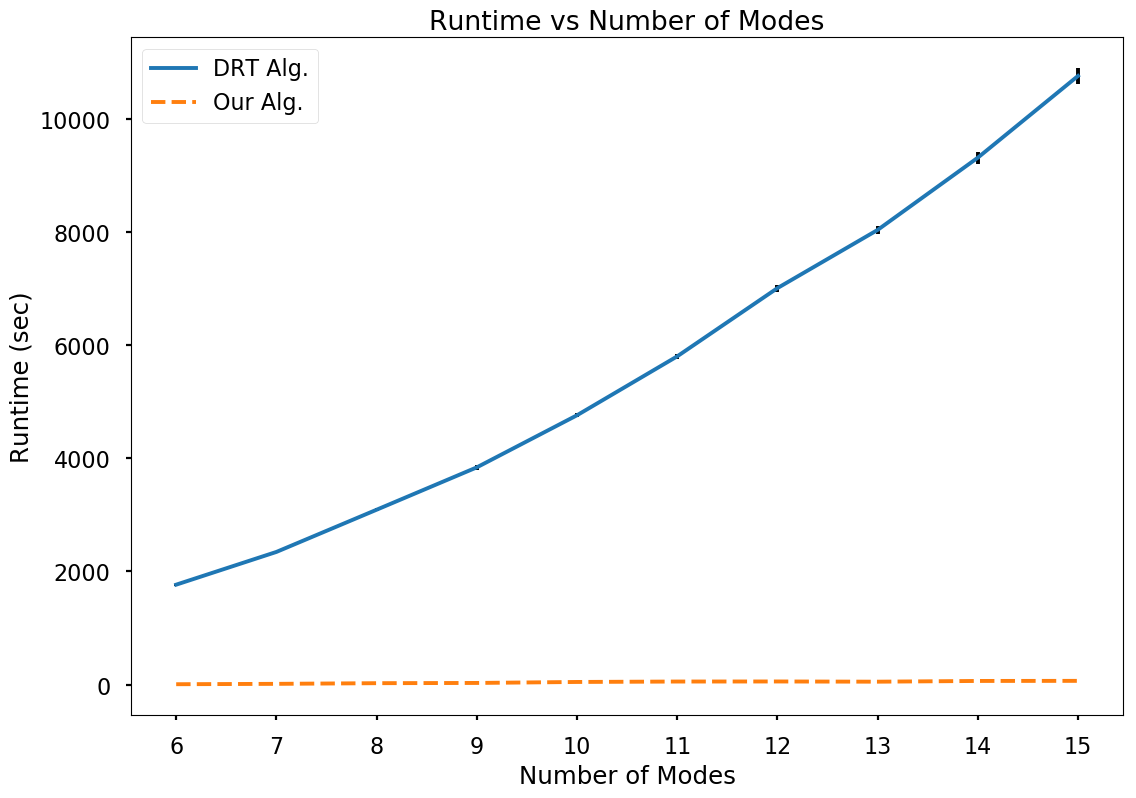
\includegraphics[width=1.0\linewidth]{Figures/runtimePlot-confidence_intervals.png}
\caption{Graph depicting the runtime of different algorithms as a function of the number of modes of randomly generated AVR task sets. For each mode, the 95\% confidence interval is shown.}
\label{fig:finalgraph}
\end{figure}

For the second experiment, we generated multiple AVR tasks using an algorithm presented by Biondi et al.~\cite{biondi_response-time_2015}. In this algorithm, multiple AVR tasks are modeled as a single task, called the representative AVR task, by combining the execution times and the boundaries speeds. The modes of the representative AVR task are generated by assuming a fixed value of 0.25 for the maximum utilization factor of the modes. Again, the same worst-case demands were found by both algorithm, but overall, our approach is 146 times faster on average and up to 250 times faster, as shown in Fig.~\ref{fig:finalgraph}.

%  \sandeep{This is how I calculated the confidence intervals and runtime averages:
%  For tasksets-1 and 2, run both the algorithms on each of the tasksets 10 times and calculate the average runtime of an algorithm per taskset. The improvement in runtime over a taskset is the ratio of the runtime average of the DRT algorithm on the given taskset and the runtime average of our algorithm on the same taskset. I do this because we have a table showing the average runtimes of our algorithm and the DRT algorithm over each of the tasksets.
%   For randomly generated tasksets: Generate 10 random tasksets each with modes 6 to 15. Run both the algorithms on each of these tasksets 10 times. Calculate the ratio of the runtime of the DRT algorithm over a taskset and the runtime of our algorithm for the corresponding run over the same taskset. The average of all the ratios (total number of averages will be 10*10=100 - each taskset has 10 averages) above gives the average improvement.
% The average runtimes and improvement ratios are calculated differently in the above two cases. Is this fine?}

\subsection{Conclusions and Future Work}
\label{sec:conclusion}

This paper presented an efficient method for calculating the exact worst-case demand bound function of AVR tasks. First, a knapsack-based dynamic programming approach was proposed to efficiently find the worst-case demand. Second, a collection of necessary conditions were presented, which reduce the search space of the knapsack-based approach to find the dominant sequence set. Experimental results confirm that the proposed approach is exact and is faster than the state-of-the-art technique. In the future, we plan on analyzing the worst-case demand of AVR tasks that have different phases and which are released by independent sources.

\subsection*{Acknowledgements.}
This research was supported in part by the US National Science Foundation (CNS Grant Nos. 1618185 \& 1618979) and a Thomas C. Rumble Graduate Fellowship from Wayne State University.


% Paper \# 1
% I <3 my Wayne State Libraries! Do you? \cite{WSULibrary}

% \paragraph{A Subsection with a Table}

% \begin{table}[!h]
%     \centering	
%     \bgroup
%     \def\arraystretch{1.00}
%     \begin{tabular}{| c | c | c | c |}
%           \hline			
%           Resource & Website & What's it for? \\ \hline \hline \cline{1-3}
%           Academic Success Center & https://success.wayne.edu/ & Academic Success!\\ \hline
%           Campus Health Center & http://health.wayne.edu/ & Health! \\ \hline
%           Writing Research and Technology Zone & http://www.clas.wayne.edu/writing/ & Writing Help!\\ \hline
%     \end{tabular}
%     \egroup
%     \caption{Wayne State University Resources}
%     \label{tab:WSUresources}
% \end{table}

% \paragraph{A Subsection with a Figure}

% \begin{figure}[!htbp]
%     \centering
%     
\includegraphics[width=0.25\linewidth]{fig/wsu_primary_stacked_color.pdf}
%     \caption{WSU Logo} The Wayne State University Logo
%     \label{fig:WSUlogo}
% \end{figure}

% \paragraph{A last Subsection}
